\documentclass[twoside]{book}

% Packages required by doxygen
\usepackage{fixltx2e}
\usepackage{calc}
\usepackage{doxygen}
\usepackage[export]{adjustbox} % also loads graphicx
\usepackage{graphicx}
\usepackage[utf8]{inputenc}
\usepackage{makeidx}
\usepackage{multicol}
\usepackage{multirow}
\PassOptionsToPackage{warn}{textcomp}
\usepackage{textcomp}
\usepackage[nointegrals]{wasysym}
\usepackage[table]{xcolor}

% NLS support packages
\usepackage[spanish]{babel}
% Font selection
\usepackage[T1]{fontenc}
\usepackage[scaled=.90]{helvet}
\usepackage{courier}
\usepackage{amssymb}
\usepackage{sectsty}
\renewcommand{\familydefault}{\sfdefault}
\allsectionsfont{%
  \fontseries{bc}\selectfont%
  \color{darkgray}%
}
\renewcommand{\DoxyLabelFont}{%
  \fontseries{bc}\selectfont%
  \color{darkgray}%
}
\newcommand{\+}{\discretionary{\mbox{\scriptsize$\hookleftarrow$}}{}{}}

% Page & text layout
\usepackage{geometry}
\geometry{%
  a4paper,%
  top=2.5cm,%
  bottom=2.5cm,%
  left=2.5cm,%
  right=2.5cm%
}
\tolerance=750
\hfuzz=15pt
\hbadness=750
\setlength{\emergencystretch}{15pt}
\setlength{\parindent}{0cm}
\setlength{\parskip}{3ex plus 2ex minus 2ex}
\makeatletter
\renewcommand{\paragraph}{%
  \@startsection{paragraph}{4}{0ex}{-1.0ex}{1.0ex}{%
    \normalfont\normalsize\bfseries\SS@parafont%
  }%
}
\renewcommand{\subparagraph}{%
  \@startsection{subparagraph}{5}{0ex}{-1.0ex}{1.0ex}{%
    \normalfont\normalsize\bfseries\SS@subparafont%
  }%
}
\makeatother

% Headers & footers
\usepackage{fancyhdr}
\pagestyle{fancyplain}
\fancyhead[LE]{\fancyplain{}{\bfseries\thepage}}
\fancyhead[CE]{\fancyplain{}{}}
\fancyhead[RE]{\fancyplain{}{\bfseries\leftmark}}
\fancyhead[LO]{\fancyplain{}{\bfseries\rightmark}}
\fancyhead[CO]{\fancyplain{}{}}
\fancyhead[RO]{\fancyplain{}{\bfseries\thepage}}
\fancyfoot[LE]{\fancyplain{}{}}
\fancyfoot[CE]{\fancyplain{}{}}
\fancyfoot[RE]{\fancyplain{}{\bfseries\scriptsize Generado por Doxygen }}
\fancyfoot[LO]{\fancyplain{}{\bfseries\scriptsize Generado por Doxygen }}
\fancyfoot[CO]{\fancyplain{}{}}
\fancyfoot[RO]{\fancyplain{}{}}
\renewcommand{\footrulewidth}{0.4pt}
\renewcommand{\chaptermark}[1]{%
  \markboth{#1}{}%
}
\renewcommand{\sectionmark}[1]{%
  \markright{\thesection\ #1}%
}

% Indices & bibliography
\usepackage{natbib}
\usepackage[titles]{tocloft}
\setcounter{tocdepth}{3}
\setcounter{secnumdepth}{5}
\makeindex

% Hyperlinks (required, but should be loaded last)
\usepackage{ifpdf}
\ifpdf
  \usepackage[pdftex,pagebackref=true]{hyperref}
\else
  \usepackage[ps2pdf,pagebackref=true]{hyperref}
\fi
\hypersetup{%
  colorlinks=true,%
  linkcolor=blue,%
  citecolor=blue,%
  unicode%
}

% Custom commands
\newcommand{\clearemptydoublepage}{%
  \newpage{\pagestyle{empty}\cleardoublepage}%
}

\usepackage{caption}
\captionsetup{labelsep=space,justification=centering,font={bf},singlelinecheck=off,skip=4pt,position=top}

%===== C O N T E N T S =====

\begin{document}

% Titlepage & ToC
\hypersetup{pageanchor=false,
             bookmarksnumbered=true,
             pdfencoding=unicode
            }
\pagenumbering{alph}
\begin{titlepage}
\vspace*{7cm}
\begin{center}%
{\Large Structure\+Visualizator \\[1ex]\large 1.\+0 }\\
\vspace*{1cm}
{\large Generado por Doxygen 1.8.14}\\
\end{center}
\end{titlepage}
\clearemptydoublepage
\pagenumbering{roman}
\tableofcontents
\clearemptydoublepage
\pagenumbering{arabic}
\hypersetup{pageanchor=true}

%--- Begin generated contents ---
\chapter{Indice de namespaces}
\section{Lista de \textquotesingle{}namespaces\textquotesingle{}}
Lista de los \textquotesingle{}namespaces\textquotesingle{}, con una breve descripción\+:\begin{DoxyCompactList}
\item\contentsline{section}{\mbox{\hyperlink{namespace_ui}{Ui}} }{\pageref{namespace_ui}}{}
\end{DoxyCompactList}

\chapter{Indice jerárquico}
\section{Jerarquía de la clase}
Esta lista de herencias esta ordenada aproximadamente por orden alfabético\+:\begin{DoxyCompactList}
\item \contentsline{section}{Binary\+Tree}{\pageref{class_binary_tree}}{}
\item \contentsline{section}{Circular\+List}{\pageref{class_circular_list}}{}
\item \contentsline{section}{Doble\+Linked\+List}{\pageref{class_doble_linked_list}}{}
\item \contentsline{section}{Nodo\+Doble\+Enlazado}{\pageref{class_nodo_doble_enlazado}}{}
\item \contentsline{section}{Nodo\+Lista\+Circular}{\pageref{class_nodo_lista_circular}}{}
\item \contentsline{section}{Nodo\+Simple}{\pageref{class_nodo_simple}}{}
\item Q\+Dialog\begin{DoxyCompactList}
\item \contentsline{section}{Enlazada\+Doble}{\pageref{class_enlazada_doble}}{}
\item \contentsline{section}{Lista\+Simple}{\pageref{class_lista_simple}}{}
\item \contentsline{section}{View\+Circular\+List}{\pageref{class_view_circular_list}}{}
\item \contentsline{section}{View\+Tree}{\pageref{class_view_tree}}{}
\end{DoxyCompactList}
\item Q\+Main\+Window\begin{DoxyCompactList}
\item \contentsline{section}{Main\+Window}{\pageref{class_main_window}}{}
\end{DoxyCompactList}
\item \contentsline{section}{Simple\+Linked\+List}{\pageref{class_simple_linked_list}}{}
\item \contentsline{section}{Tree\+Node}{\pageref{class_tree_node}}{}
\end{DoxyCompactList}

\chapter{Índice de clases}
\section{Lista de clases}
Lista de las clases, estructuras, uniones e interfaces con una breve descripción\+:\begin{DoxyCompactList}
\item\contentsline{section}{\mbox{\hyperlink{class_binary_tree}{Binary\+Tree}} \\*Clase que maneja la estructura del arbol binario }{\pageref{class_binary_tree}}{}
\item\contentsline{section}{\mbox{\hyperlink{class_circular_list}{Circular\+List}} \\*Clase que contiene la estructura de datos de la lista circular }{\pageref{class_circular_list}}{}
\item\contentsline{section}{\mbox{\hyperlink{class_doble_linked_list}{Doble\+Linked\+List}} \\*Clase que contiene la estructura de las listas doblemente enlazadas }{\pageref{class_doble_linked_list}}{}
\item\contentsline{section}{\mbox{\hyperlink{class_enlazada_doble}{Enlazada\+Doble}} \\*Clase que contiene lo referente a la ventana de la lista doblemente enlazada }{\pageref{class_enlazada_doble}}{}
\item\contentsline{section}{\mbox{\hyperlink{class_lista_simple}{Lista\+Simple}} \\*Clase que contiene lo referente a la ventana de la lista simple }{\pageref{class_lista_simple}}{}
\item\contentsline{section}{\mbox{\hyperlink{class_main_window}{Main\+Window}} \\*Esta clase controla todo lo referente a lo que se encuentra en la ventana inicial }{\pageref{class_main_window}}{}
\item\contentsline{section}{\mbox{\hyperlink{class_nodo_doble_enlazado}{Nodo\+Doble\+Enlazado}} \\*Estructura de datos nodo para lista doble enlazada }{\pageref{class_nodo_doble_enlazado}}{}
\item\contentsline{section}{\mbox{\hyperlink{class_nodo_lista_circular}{Nodo\+Lista\+Circular}} \\*Estructura del nodo de la lista circular }{\pageref{class_nodo_lista_circular}}{}
\item\contentsline{section}{\mbox{\hyperlink{class_nodo_simple}{Nodo\+Simple}} \\*Estructura del nodo de la lista simple }{\pageref{class_nodo_simple}}{}
\item\contentsline{section}{\mbox{\hyperlink{class_simple_linked_list}{Simple\+Linked\+List}} \\*Estructura de la lista simple }{\pageref{class_simple_linked_list}}{}
\item\contentsline{section}{\mbox{\hyperlink{class_tree_node}{Tree\+Node}} \\*Estructura del nodo para el arbol }{\pageref{class_tree_node}}{}
\item\contentsline{section}{\mbox{\hyperlink{class_view_circular_list}{View\+Circular\+List}} \\*Ventana De la Lista Circular }{\pageref{class_view_circular_list}}{}
\item\contentsline{section}{\mbox{\hyperlink{class_view_tree}{View\+Tree}} \\*Clase que se encarga de la ventana del Arbol binario }{\pageref{class_view_tree}}{}
\end{DoxyCompactList}

\chapter{Indice de archivos}
\section{Lista de archivos}
Lista de todos los archivos con descripciones breves\+:\begin{DoxyCompactList}
\item\contentsline{section}{\mbox{\hyperlink{binarytree_8h}{binarytree.\+h}} \\*Archivo que tiene lo referente al arbol binario }{\pageref{binarytree_8h}}{}
\item\contentsline{section}{\mbox{\hyperlink{circularlist_8h}{circularlist.\+h}} \\*Estructura de datos lista circular }{\pageref{circularlist_8h}}{}
\item\contentsline{section}{\mbox{\hyperlink{doblelinkedlist_8h}{doblelinkedlist.\+h}} \\*Estructura de datos lista doblemente enlanzada }{\pageref{doblelinkedlist_8h}}{}
\item\contentsline{section}{\mbox{\hyperlink{enlazadadoble_8cpp}{enlazadadoble.\+cpp}} }{\pageref{enlazadadoble_8cpp}}{}
\item\contentsline{section}{\mbox{\hyperlink{enlazadadoble_8h}{enlazadadoble.\+h}} \\*Contiene lo referente a la ventana de la lista doblemente enlazada }{\pageref{enlazadadoble_8h}}{}
\item\contentsline{section}{\mbox{\hyperlink{listasimple_8cpp}{listasimple.\+cpp}} }{\pageref{listasimple_8cpp}}{}
\item\contentsline{section}{\mbox{\hyperlink{listasimple_8h}{listasimple.\+h}} \\*Contiene lo referente a la ventana de la lista simple }{\pageref{listasimple_8h}}{}
\item\contentsline{section}{\mbox{\hyperlink{main_8cpp}{main.\+cpp}} }{\pageref{main_8cpp}}{}
\item\contentsline{section}{\mbox{\hyperlink{mainwindow_8cpp}{mainwindow.\+cpp}} }{\pageref{mainwindow_8cpp}}{}
\item\contentsline{section}{\mbox{\hyperlink{mainwindow_8h}{mainwindow.\+h}} \\*Controla todo lo referente a lo que se encuentra en la ventana principal }{\pageref{mainwindow_8h}}{}
\item\contentsline{section}{\mbox{\hyperlink{nododobleenlazado_8h}{nododobleenlazado.\+h}} \\*Estructura de datos nodo para lista doble enlazada }{\pageref{nododobleenlazado_8h}}{}
\item\contentsline{section}{\mbox{\hyperlink{nodolistacircular_8h}{nodolistacircular.\+h}} \\*Estructura del nodo de la lista circular }{\pageref{nodolistacircular_8h}}{}
\item\contentsline{section}{\mbox{\hyperlink{nodosimple_8h}{nodosimple.\+h}} \\*Estructura del nodo de la lista simple }{\pageref{nodosimple_8h}}{}
\item\contentsline{section}{\mbox{\hyperlink{simplelinkedlist_8h}{simplelinkedlist.\+h}} \\*Estructura de la lista simple }{\pageref{simplelinkedlist_8h}}{}
\item\contentsline{section}{\mbox{\hyperlink{treenode_8h}{treenode.\+h}} \\*Estructura del nodo para el arbol }{\pageref{treenode_8h}}{}
\item\contentsline{section}{\mbox{\hyperlink{viewcircularlist_8cpp}{viewcircularlist.\+cpp}} }{\pageref{viewcircularlist_8cpp}}{}
\item\contentsline{section}{\mbox{\hyperlink{viewcircularlist_8h}{viewcircularlist.\+h}} \\*Controla todo lo referente a la ventana De la Lista Circular }{\pageref{viewcircularlist_8h}}{}
\item\contentsline{section}{\mbox{\hyperlink{viewtree_8cpp}{viewtree.\+cpp}} }{\pageref{viewtree_8cpp}}{}
\item\contentsline{section}{\mbox{\hyperlink{viewtree_8h}{viewtree.\+h}} \\*Contiene todo lo referente a la ventana del arbol binario }{\pageref{viewtree_8h}}{}
\end{DoxyCompactList}

\chapter{Documentación de namespaces}
\hypertarget{namespace_ui}{}\section{Referencia del Namespace Ui}
\label{namespace_ui}\index{Ui@{Ui}}

\chapter{Documentación de las clases}
\hypertarget{class_binary_tree}{}\section{Referencia de la Clase Binary\+Tree}
\label{class_binary_tree}\index{Binary\+Tree@{Binary\+Tree}}


The \mbox{\hyperlink{class_binary_tree}{Binary\+Tree}} class clase que maneja la estructura del arbol binario.  




{\ttfamily \#include $<$binarytree.\+h$>$}

\subsection*{Métodos públicos}
\begin{DoxyCompactItemize}
\item 
\mbox{\hyperlink{class_binary_tree_adf45bce605436b26c353b87e27bffe50}{Binary\+Tree}} ()
\begin{DoxyCompactList}\small\item\em \mbox{\hyperlink{class_binary_tree}{Binary\+Tree}} inicia el arbol binario. \end{DoxyCompactList}\item 
\mbox{\hyperlink{class_tree_node}{Tree\+Node}} $\ast$ \mbox{\hyperlink{class_binary_tree_aabfed860b1c67b2a1cd12eacf870fc8c}{get\+Root}} ()
\item 
void \mbox{\hyperlink{class_binary_tree_a198bb1b6bd9d4fe1535d8189b9d3dc3e}{insertar\+Nodo}} (int dato)
\begin{DoxyCompactList}\small\item\em insertar\+Nodo inserta un nodo \end{DoxyCompactList}\item 
void \mbox{\hyperlink{class_binary_tree_ad7162208805ed8f96c59cc6ba47d25a1}{recorrido\+Pre\+Order}} (\mbox{\hyperlink{class_tree_node}{Tree\+Node}} $\ast$nodo)
\begin{DoxyCompactList}\small\item\em recorrido\+Pre\+Order es el dato del nodo \end{DoxyCompactList}\item 
void \mbox{\hyperlink{class_binary_tree_a457aa0a390da80c9d732c525dd006d0f}{eliminar}} (\mbox{\hyperlink{class_tree_node}{Tree\+Node}} $\ast$nodo, int buscado)
\begin{DoxyCompactList}\small\item\em eliminar busca el nodo que se quiere eliminar \end{DoxyCompactList}\item 
void \mbox{\hyperlink{class_binary_tree_ae67035ec37e83ccbceabb71826226e8d}{eliminar\+Nodo}} (\mbox{\hyperlink{class_tree_node}{Tree\+Node}} $\ast$nodo)
\begin{DoxyCompactList}\small\item\em eliminar\+Nodo cambia las referencias del nodo para poder eliminarlo \end{DoxyCompactList}\item 
\mbox{\hyperlink{class_tree_node}{Tree\+Node}} $\ast$ \mbox{\hyperlink{class_binary_tree_abcee209ca30b59708c0ef9f22863944c}{minimo}} (\mbox{\hyperlink{class_tree_node}{Tree\+Node}} $\ast$nodo)
\begin{DoxyCompactList}\small\item\em minimo busca el nodo por el cual se va a remplazar \end{DoxyCompactList}\item 
void \mbox{\hyperlink{class_binary_tree_a9fe0609a3ea42f1e3062e25e43fea81b}{remplazar}} (\mbox{\hyperlink{class_tree_node}{Tree\+Node}} $\ast$nodo, \mbox{\hyperlink{class_tree_node}{Tree\+Node}} $\ast$nodonuevo)
\begin{DoxyCompactList}\small\item\em remplazar remplaza el nodo que se busca por el minimo a su derecha \end{DoxyCompactList}\item 
void \mbox{\hyperlink{class_binary_tree_adca59e6c9ff7a3c87aa35955ba7897ef}{destroy}} (\mbox{\hyperlink{class_tree_node}{Tree\+Node}} $\ast$node)
\begin{DoxyCompactList}\small\item\em destroy elimina el nodo cambiadole las referencias \end{DoxyCompactList}\end{DoxyCompactItemize}


\subsection{Descripción detallada}
The \mbox{\hyperlink{class_binary_tree}{Binary\+Tree}} class clase que maneja la estructura del arbol binario. 

\subsection{Documentación del constructor y destructor}
\mbox{\Hypertarget{class_binary_tree_adf45bce605436b26c353b87e27bffe50}\label{class_binary_tree_adf45bce605436b26c353b87e27bffe50}} 
\index{Binary\+Tree@{Binary\+Tree}!Binary\+Tree@{Binary\+Tree}}
\index{Binary\+Tree@{Binary\+Tree}!Binary\+Tree@{Binary\+Tree}}
\subsubsection{\texorpdfstring{Binary\+Tree()}{BinaryTree()}}
{\footnotesize\ttfamily Binary\+Tree\+::\+Binary\+Tree (\begin{DoxyParamCaption}{ }\end{DoxyParamCaption})\hspace{0.3cm}{\ttfamily [inline]}}



\mbox{\hyperlink{class_binary_tree}{Binary\+Tree}} inicia el arbol binario. 



\subsection{Documentación de las funciones miembro}
\mbox{\Hypertarget{class_binary_tree_adca59e6c9ff7a3c87aa35955ba7897ef}\label{class_binary_tree_adca59e6c9ff7a3c87aa35955ba7897ef}} 
\index{Binary\+Tree@{Binary\+Tree}!destroy@{destroy}}
\index{destroy@{destroy}!Binary\+Tree@{Binary\+Tree}}
\subsubsection{\texorpdfstring{destroy()}{destroy()}}
{\footnotesize\ttfamily void Binary\+Tree\+::destroy (\begin{DoxyParamCaption}\item[{\mbox{\hyperlink{class_tree_node}{Tree\+Node}} $\ast$}]{node }\end{DoxyParamCaption})\hspace{0.3cm}{\ttfamily [inline]}}



destroy elimina el nodo cambiadole las referencias 


\begin{DoxyParams}{Parámetros}
{\em node} & el nodo a eliminar \\
\hline
\end{DoxyParams}
\mbox{\Hypertarget{class_binary_tree_a457aa0a390da80c9d732c525dd006d0f}\label{class_binary_tree_a457aa0a390da80c9d732c525dd006d0f}} 
\index{Binary\+Tree@{Binary\+Tree}!eliminar@{eliminar}}
\index{eliminar@{eliminar}!Binary\+Tree@{Binary\+Tree}}
\subsubsection{\texorpdfstring{eliminar()}{eliminar()}}
{\footnotesize\ttfamily void Binary\+Tree\+::eliminar (\begin{DoxyParamCaption}\item[{\mbox{\hyperlink{class_tree_node}{Tree\+Node}} $\ast$}]{nodo,  }\item[{int}]{buscado }\end{DoxyParamCaption})\hspace{0.3cm}{\ttfamily [inline]}}



eliminar busca el nodo que se quiere eliminar 


\begin{DoxyParams}{Parámetros}
{\em nodo} & nodo por el que se esta recorriendo \\
\hline
{\em buscado} & valor entero que determina el valor buscado \\
\hline
\end{DoxyParams}
\mbox{\Hypertarget{class_binary_tree_ae67035ec37e83ccbceabb71826226e8d}\label{class_binary_tree_ae67035ec37e83ccbceabb71826226e8d}} 
\index{Binary\+Tree@{Binary\+Tree}!eliminar\+Nodo@{eliminar\+Nodo}}
\index{eliminar\+Nodo@{eliminar\+Nodo}!Binary\+Tree@{Binary\+Tree}}
\subsubsection{\texorpdfstring{eliminar\+Nodo()}{eliminarNodo()}}
{\footnotesize\ttfamily void Binary\+Tree\+::eliminar\+Nodo (\begin{DoxyParamCaption}\item[{\mbox{\hyperlink{class_tree_node}{Tree\+Node}} $\ast$}]{nodo }\end{DoxyParamCaption})\hspace{0.3cm}{\ttfamily [inline]}}



eliminar\+Nodo cambia las referencias del nodo para poder eliminarlo 


\begin{DoxyParams}{Parámetros}
{\em nodo} & nodo que se elimina \\
\hline
\end{DoxyParams}
\mbox{\Hypertarget{class_binary_tree_aabfed860b1c67b2a1cd12eacf870fc8c}\label{class_binary_tree_aabfed860b1c67b2a1cd12eacf870fc8c}} 
\index{Binary\+Tree@{Binary\+Tree}!get\+Root@{get\+Root}}
\index{get\+Root@{get\+Root}!Binary\+Tree@{Binary\+Tree}}
\subsubsection{\texorpdfstring{get\+Root()}{getRoot()}}
{\footnotesize\ttfamily \mbox{\hyperlink{class_tree_node}{Tree\+Node}}$\ast$ Binary\+Tree\+::get\+Root (\begin{DoxyParamCaption}{ }\end{DoxyParamCaption})\hspace{0.3cm}{\ttfamily [inline]}}

\mbox{\Hypertarget{class_binary_tree_a198bb1b6bd9d4fe1535d8189b9d3dc3e}\label{class_binary_tree_a198bb1b6bd9d4fe1535d8189b9d3dc3e}} 
\index{Binary\+Tree@{Binary\+Tree}!insertar\+Nodo@{insertar\+Nodo}}
\index{insertar\+Nodo@{insertar\+Nodo}!Binary\+Tree@{Binary\+Tree}}
\subsubsection{\texorpdfstring{insertar\+Nodo()}{insertarNodo()}}
{\footnotesize\ttfamily void Binary\+Tree\+::insertar\+Nodo (\begin{DoxyParamCaption}\item[{int}]{dato }\end{DoxyParamCaption})\hspace{0.3cm}{\ttfamily [inline]}}



insertar\+Nodo inserta un nodo 


\begin{DoxyParams}{Parámetros}
{\em dato} & es el dato del nodo \\
\hline
\end{DoxyParams}
\mbox{\Hypertarget{class_binary_tree_abcee209ca30b59708c0ef9f22863944c}\label{class_binary_tree_abcee209ca30b59708c0ef9f22863944c}} 
\index{Binary\+Tree@{Binary\+Tree}!minimo@{minimo}}
\index{minimo@{minimo}!Binary\+Tree@{Binary\+Tree}}
\subsubsection{\texorpdfstring{minimo()}{minimo()}}
{\footnotesize\ttfamily \mbox{\hyperlink{class_tree_node}{Tree\+Node}}$\ast$ Binary\+Tree\+::minimo (\begin{DoxyParamCaption}\item[{\mbox{\hyperlink{class_tree_node}{Tree\+Node}} $\ast$}]{nodo }\end{DoxyParamCaption})\hspace{0.3cm}{\ttfamily [inline]}}



minimo busca el nodo por el cual se va a remplazar 


\begin{DoxyParams}{Parámetros}
{\em nodo} & nodo por el cual se va recorriendo \\
\hline
\end{DoxyParams}
\begin{DoxyReturn}{Devuelve}
retorna el nodopor el cual se va a sustituir 
\end{DoxyReturn}
\mbox{\Hypertarget{class_binary_tree_ad7162208805ed8f96c59cc6ba47d25a1}\label{class_binary_tree_ad7162208805ed8f96c59cc6ba47d25a1}} 
\index{Binary\+Tree@{Binary\+Tree}!recorrido\+Pre\+Order@{recorrido\+Pre\+Order}}
\index{recorrido\+Pre\+Order@{recorrido\+Pre\+Order}!Binary\+Tree@{Binary\+Tree}}
\subsubsection{\texorpdfstring{recorrido\+Pre\+Order()}{recorridoPreOrder()}}
{\footnotesize\ttfamily void Binary\+Tree\+::recorrido\+Pre\+Order (\begin{DoxyParamCaption}\item[{\mbox{\hyperlink{class_tree_node}{Tree\+Node}} $\ast$}]{nodo }\end{DoxyParamCaption})\hspace{0.3cm}{\ttfamily [inline]}}



recorrido\+Pre\+Order es el dato del nodo 


\begin{DoxyParams}{Parámetros}
{\em nodo} & nodo incial desde donde se va a recorrer \\
\hline
\end{DoxyParams}
\mbox{\Hypertarget{class_binary_tree_a9fe0609a3ea42f1e3062e25e43fea81b}\label{class_binary_tree_a9fe0609a3ea42f1e3062e25e43fea81b}} 
\index{Binary\+Tree@{Binary\+Tree}!remplazar@{remplazar}}
\index{remplazar@{remplazar}!Binary\+Tree@{Binary\+Tree}}
\subsubsection{\texorpdfstring{remplazar()}{remplazar()}}
{\footnotesize\ttfamily void Binary\+Tree\+::remplazar (\begin{DoxyParamCaption}\item[{\mbox{\hyperlink{class_tree_node}{Tree\+Node}} $\ast$}]{nodo,  }\item[{\mbox{\hyperlink{class_tree_node}{Tree\+Node}} $\ast$}]{nodonuevo }\end{DoxyParamCaption})\hspace{0.3cm}{\ttfamily [inline]}}



remplazar remplaza el nodo que se busca por el minimo a su derecha 


\begin{DoxyParams}{Parámetros}
{\em nodo} & nodo que se va a elimianr \\
\hline
{\em nodonuevo} & nodo \\
\hline
\end{DoxyParams}


La documentación para esta clase fue generada a partir del siguiente fichero\+:\begin{DoxyCompactItemize}
\item 
\mbox{\hyperlink{binarytree_8h}{binarytree.\+h}}\end{DoxyCompactItemize}

\hypertarget{class_circular_list}{}\section{Referencia de la Clase Circular\+List}
\label{class_circular_list}\index{Circular\+List@{Circular\+List}}


The \mbox{\hyperlink{class_circular_list}{Circular\+List}} class clase que contiene la estructura de datos de la lista circular.  




{\ttfamily \#include $<$circularlist.\+h$>$}

\subsection*{Métodos públicos}
\begin{DoxyCompactItemize}
\item 
\mbox{\hyperlink{class_circular_list_ad4877c840f41f3119b1378e7ac35386c}{Circular\+List}} ()
\begin{DoxyCompactList}\small\item\em \mbox{\hyperlink{class_circular_list}{Circular\+List}} inicia la lista circular. \end{DoxyCompactList}\item 
void \mbox{\hyperlink{class_circular_list_a4d9c44a0352121d91be126746b48408f}{ingresar\+Dato\+Final}} (Q\+String dato)
\begin{DoxyCompactList}\small\item\em ingresar\+Dato\+Final ingresa un dato al final de la lista \end{DoxyCompactList}\item 
void \mbox{\hyperlink{class_circular_list_a4d498cd4c405704101003b90d782bb93}{ingresar\+Dato\+Inicio}} (Q\+String dato)
\begin{DoxyCompactList}\small\item\em ingresar\+Dato\+Inicio ingresa un dato al inicio \end{DoxyCompactList}\item 
void \mbox{\hyperlink{class_circular_list_ad2dd3f4b5934900494ba50714306a89f}{insertar\+Por\+Posicion}} (int pos, Q\+String dato)
\begin{DoxyCompactList}\small\item\em insertar\+Por\+Posicion inserta un nodo en la lista por su posicion \end{DoxyCompactList}\item 
void \mbox{\hyperlink{class_circular_list_a7cf69aaaf998bac2f5342da4adc5e55d}{eliminar\+Posicion}} (int pos)
\begin{DoxyCompactList}\small\item\em eliminar\+Posicion eliminar un nodo por posicion \end{DoxyCompactList}\item 
void \mbox{\hyperlink{class_circular_list_a3a3c9755cb691e9b02f6d584f2fd1c8e}{eliminar\+Inicio}} ()
\begin{DoxyCompactList}\small\item\em eliminar\+Inicio elimina el nodo inicial de la lista \end{DoxyCompactList}\item 
void \mbox{\hyperlink{class_circular_list_a65808e0225fce3f7b90a70973adfc0ff}{eliminar\+Final}} ()
\begin{DoxyCompactList}\small\item\em eliminar\+Final elimina el nodo final de la lista \end{DoxyCompactList}\item 
void \mbox{\hyperlink{class_circular_list_a731a6238e742307bcd2734ba90ec360f}{imprimir\+Lista\+Al\+Derecho}} ()
\begin{DoxyCompactList}\small\item\em imprimir\+Lista\+Al\+Derecho imprime la lista de inicio a fin \end{DoxyCompactList}\item 
void \mbox{\hyperlink{class_circular_list_a5f98eb44e45979a6373ad7abda059d44}{editar}} (int pos, Q\+String dato)
\begin{DoxyCompactList}\small\item\em editar cambia el valor de un nodo en especifico \end{DoxyCompactList}\item 
\mbox{\hyperlink{class_nodo_lista_circular}{Nodo\+Lista\+Circular}} \mbox{\hyperlink{class_circular_list_abc60af99960852c2aecfc352dd55f48e}{obtenerpor\+Posicion}} (int pos)
\begin{DoxyCompactList}\small\item\em obtenerpor\+Posicion retorna el nodo que se especifica en la posicion \end{DoxyCompactList}\end{DoxyCompactItemize}
\subsection*{Atributos públicos}
\begin{DoxyCompactItemize}
\item 
\mbox{\hyperlink{class_nodo_lista_circular}{Nodo\+Lista\+Circular}} $\ast$ \mbox{\hyperlink{class_circular_list_aed38c338f4196ea0eb66f3990b7f3bc8}{primero}}
\item 
\mbox{\hyperlink{class_nodo_lista_circular}{Nodo\+Lista\+Circular}} $\ast$ \mbox{\hyperlink{class_circular_list_a45e599ae210b5ebc41a5cd9149bce79e}{ultimo}}
\item 
int \mbox{\hyperlink{class_circular_list_ab94765d81b2b6bd145abdb7dad48339e}{largo}} = 0
\end{DoxyCompactItemize}


\subsection{Descripción detallada}
The \mbox{\hyperlink{class_circular_list}{Circular\+List}} class clase que contiene la estructura de datos de la lista circular. 

\subsection{Documentación del constructor y destructor}
\mbox{\Hypertarget{class_circular_list_ad4877c840f41f3119b1378e7ac35386c}\label{class_circular_list_ad4877c840f41f3119b1378e7ac35386c}} 
\index{Circular\+List@{Circular\+List}!Circular\+List@{Circular\+List}}
\index{Circular\+List@{Circular\+List}!Circular\+List@{Circular\+List}}
\subsubsection{\texorpdfstring{Circular\+List()}{CircularList()}}
{\footnotesize\ttfamily Circular\+List\+::\+Circular\+List (\begin{DoxyParamCaption}{ }\end{DoxyParamCaption})\hspace{0.3cm}{\ttfamily [inline]}}



\mbox{\hyperlink{class_circular_list}{Circular\+List}} inicia la lista circular. 



\subsection{Documentación de las funciones miembro}
\mbox{\Hypertarget{class_circular_list_a5f98eb44e45979a6373ad7abda059d44}\label{class_circular_list_a5f98eb44e45979a6373ad7abda059d44}} 
\index{Circular\+List@{Circular\+List}!editar@{editar}}
\index{editar@{editar}!Circular\+List@{Circular\+List}}
\subsubsection{\texorpdfstring{editar()}{editar()}}
{\footnotesize\ttfamily void Circular\+List\+::editar (\begin{DoxyParamCaption}\item[{int}]{pos,  }\item[{Q\+String}]{dato }\end{DoxyParamCaption})\hspace{0.3cm}{\ttfamily [inline]}}



editar cambia el valor de un nodo en especifico 


\begin{DoxyParams}{Parámetros}
{\em pos} & la posicion del nodo que se quiere editar \\
\hline
{\em dato} & dato nuevo que se le quiere dar \\
\hline
\end{DoxyParams}
\mbox{\Hypertarget{class_circular_list_a65808e0225fce3f7b90a70973adfc0ff}\label{class_circular_list_a65808e0225fce3f7b90a70973adfc0ff}} 
\index{Circular\+List@{Circular\+List}!eliminar\+Final@{eliminar\+Final}}
\index{eliminar\+Final@{eliminar\+Final}!Circular\+List@{Circular\+List}}
\subsubsection{\texorpdfstring{eliminar\+Final()}{eliminarFinal()}}
{\footnotesize\ttfamily void Circular\+List\+::eliminar\+Final (\begin{DoxyParamCaption}{ }\end{DoxyParamCaption})\hspace{0.3cm}{\ttfamily [inline]}}



eliminar\+Final elimina el nodo final de la lista 

\mbox{\Hypertarget{class_circular_list_a3a3c9755cb691e9b02f6d584f2fd1c8e}\label{class_circular_list_a3a3c9755cb691e9b02f6d584f2fd1c8e}} 
\index{Circular\+List@{Circular\+List}!eliminar\+Inicio@{eliminar\+Inicio}}
\index{eliminar\+Inicio@{eliminar\+Inicio}!Circular\+List@{Circular\+List}}
\subsubsection{\texorpdfstring{eliminar\+Inicio()}{eliminarInicio()}}
{\footnotesize\ttfamily void Circular\+List\+::eliminar\+Inicio (\begin{DoxyParamCaption}{ }\end{DoxyParamCaption})\hspace{0.3cm}{\ttfamily [inline]}}



eliminar\+Inicio elimina el nodo inicial de la lista 

\mbox{\Hypertarget{class_circular_list_a7cf69aaaf998bac2f5342da4adc5e55d}\label{class_circular_list_a7cf69aaaf998bac2f5342da4adc5e55d}} 
\index{Circular\+List@{Circular\+List}!eliminar\+Posicion@{eliminar\+Posicion}}
\index{eliminar\+Posicion@{eliminar\+Posicion}!Circular\+List@{Circular\+List}}
\subsubsection{\texorpdfstring{eliminar\+Posicion()}{eliminarPosicion()}}
{\footnotesize\ttfamily void Circular\+List\+::eliminar\+Posicion (\begin{DoxyParamCaption}\item[{int}]{pos }\end{DoxyParamCaption})\hspace{0.3cm}{\ttfamily [inline]}}



eliminar\+Posicion eliminar un nodo por posicion 


\begin{DoxyParams}{Parámetros}
{\em pos} & posicion del nodo que se quiere eliminar \\
\hline
\end{DoxyParams}
\mbox{\Hypertarget{class_circular_list_a731a6238e742307bcd2734ba90ec360f}\label{class_circular_list_a731a6238e742307bcd2734ba90ec360f}} 
\index{Circular\+List@{Circular\+List}!imprimir\+Lista\+Al\+Derecho@{imprimir\+Lista\+Al\+Derecho}}
\index{imprimir\+Lista\+Al\+Derecho@{imprimir\+Lista\+Al\+Derecho}!Circular\+List@{Circular\+List}}
\subsubsection{\texorpdfstring{imprimir\+Lista\+Al\+Derecho()}{imprimirListaAlDerecho()}}
{\footnotesize\ttfamily void Circular\+List\+::imprimir\+Lista\+Al\+Derecho (\begin{DoxyParamCaption}{ }\end{DoxyParamCaption})\hspace{0.3cm}{\ttfamily [inline]}}



imprimir\+Lista\+Al\+Derecho imprime la lista de inicio a fin 

\mbox{\Hypertarget{class_circular_list_a4d9c44a0352121d91be126746b48408f}\label{class_circular_list_a4d9c44a0352121d91be126746b48408f}} 
\index{Circular\+List@{Circular\+List}!ingresar\+Dato\+Final@{ingresar\+Dato\+Final}}
\index{ingresar\+Dato\+Final@{ingresar\+Dato\+Final}!Circular\+List@{Circular\+List}}
\subsubsection{\texorpdfstring{ingresar\+Dato\+Final()}{ingresarDatoFinal()}}
{\footnotesize\ttfamily void Circular\+List\+::ingresar\+Dato\+Final (\begin{DoxyParamCaption}\item[{Q\+String}]{dato }\end{DoxyParamCaption})\hspace{0.3cm}{\ttfamily [inline]}}



ingresar\+Dato\+Final ingresa un dato al final de la lista 


\begin{DoxyParams}{Parámetros}
{\em dato} & es un Q\+String que es el dato del nodo \\
\hline
\end{DoxyParams}
\mbox{\Hypertarget{class_circular_list_a4d498cd4c405704101003b90d782bb93}\label{class_circular_list_a4d498cd4c405704101003b90d782bb93}} 
\index{Circular\+List@{Circular\+List}!ingresar\+Dato\+Inicio@{ingresar\+Dato\+Inicio}}
\index{ingresar\+Dato\+Inicio@{ingresar\+Dato\+Inicio}!Circular\+List@{Circular\+List}}
\subsubsection{\texorpdfstring{ingresar\+Dato\+Inicio()}{ingresarDatoInicio()}}
{\footnotesize\ttfamily void Circular\+List\+::ingresar\+Dato\+Inicio (\begin{DoxyParamCaption}\item[{Q\+String}]{dato }\end{DoxyParamCaption})\hspace{0.3cm}{\ttfamily [inline]}}



ingresar\+Dato\+Inicio ingresa un dato al inicio 


\begin{DoxyParams}{Parámetros}
{\em dato} & el dato del nodo \\
\hline
\end{DoxyParams}
\mbox{\Hypertarget{class_circular_list_ad2dd3f4b5934900494ba50714306a89f}\label{class_circular_list_ad2dd3f4b5934900494ba50714306a89f}} 
\index{Circular\+List@{Circular\+List}!insertar\+Por\+Posicion@{insertar\+Por\+Posicion}}
\index{insertar\+Por\+Posicion@{insertar\+Por\+Posicion}!Circular\+List@{Circular\+List}}
\subsubsection{\texorpdfstring{insertar\+Por\+Posicion()}{insertarPorPosicion()}}
{\footnotesize\ttfamily void Circular\+List\+::insertar\+Por\+Posicion (\begin{DoxyParamCaption}\item[{int}]{pos,  }\item[{Q\+String}]{dato }\end{DoxyParamCaption})\hspace{0.3cm}{\ttfamily [inline]}}



insertar\+Por\+Posicion inserta un nodo en la lista por su posicion 


\begin{DoxyParams}{Parámetros}
{\em pos} & entero que especifica la posicion en la que se quiere insertar \\
\hline
{\em dato} & dato que se le quiere dar al nodo insertado \\
\hline
\end{DoxyParams}
\mbox{\Hypertarget{class_circular_list_abc60af99960852c2aecfc352dd55f48e}\label{class_circular_list_abc60af99960852c2aecfc352dd55f48e}} 
\index{Circular\+List@{Circular\+List}!obtenerpor\+Posicion@{obtenerpor\+Posicion}}
\index{obtenerpor\+Posicion@{obtenerpor\+Posicion}!Circular\+List@{Circular\+List}}
\subsubsection{\texorpdfstring{obtenerpor\+Posicion()}{obtenerporPosicion()}}
{\footnotesize\ttfamily \mbox{\hyperlink{class_nodo_lista_circular}{Nodo\+Lista\+Circular}} Circular\+List\+::obtenerpor\+Posicion (\begin{DoxyParamCaption}\item[{int}]{pos }\end{DoxyParamCaption})\hspace{0.3cm}{\ttfamily [inline]}}



obtenerpor\+Posicion retorna el nodo que se especifica en la posicion 


\begin{DoxyParams}{Parámetros}
{\em pos} & posicion del nodo que se quiere retornar \\
\hline
\end{DoxyParams}
\begin{DoxyReturn}{Devuelve}

\end{DoxyReturn}


\subsection{Documentación de los datos miembro}
\mbox{\Hypertarget{class_circular_list_ab94765d81b2b6bd145abdb7dad48339e}\label{class_circular_list_ab94765d81b2b6bd145abdb7dad48339e}} 
\index{Circular\+List@{Circular\+List}!largo@{largo}}
\index{largo@{largo}!Circular\+List@{Circular\+List}}
\subsubsection{\texorpdfstring{largo}{largo}}
{\footnotesize\ttfamily int Circular\+List\+::largo = 0}

\mbox{\Hypertarget{class_circular_list_aed38c338f4196ea0eb66f3990b7f3bc8}\label{class_circular_list_aed38c338f4196ea0eb66f3990b7f3bc8}} 
\index{Circular\+List@{Circular\+List}!primero@{primero}}
\index{primero@{primero}!Circular\+List@{Circular\+List}}
\subsubsection{\texorpdfstring{primero}{primero}}
{\footnotesize\ttfamily \mbox{\hyperlink{class_nodo_lista_circular}{Nodo\+Lista\+Circular}}$\ast$ Circular\+List\+::primero}

\mbox{\Hypertarget{class_circular_list_a45e599ae210b5ebc41a5cd9149bce79e}\label{class_circular_list_a45e599ae210b5ebc41a5cd9149bce79e}} 
\index{Circular\+List@{Circular\+List}!ultimo@{ultimo}}
\index{ultimo@{ultimo}!Circular\+List@{Circular\+List}}
\subsubsection{\texorpdfstring{ultimo}{ultimo}}
{\footnotesize\ttfamily \mbox{\hyperlink{class_nodo_lista_circular}{Nodo\+Lista\+Circular}}$\ast$ Circular\+List\+::ultimo}



La documentación para esta clase fue generada a partir del siguiente fichero\+:\begin{DoxyCompactItemize}
\item 
\mbox{\hyperlink{circularlist_8h}{circularlist.\+h}}\end{DoxyCompactItemize}

\hypertarget{class_doble_linked_list}{}\section{Referencia de la Clase Doble\+Linked\+List}
\label{class_doble_linked_list}\index{Doble\+Linked\+List@{Doble\+Linked\+List}}


The \mbox{\hyperlink{class_doble_linked_list}{Doble\+Linked\+List}} class clase que contiene la estructura de las listas doblemente enlazadas.  




{\ttfamily \#include $<$doblelinkedlist.\+h$>$}

\subsection*{Métodos públicos}
\begin{DoxyCompactItemize}
\item 
\mbox{\hyperlink{class_doble_linked_list_ae9672b17f11b4594112e9aa0166564ba}{Doble\+Linked\+List}} ()
\begin{DoxyCompactList}\small\item\em \mbox{\hyperlink{class_doble_linked_list}{Doble\+Linked\+List}} inicia la lista enlazada. \end{DoxyCompactList}\item 
void \mbox{\hyperlink{class_doble_linked_list_a856a0628fb4f272a1609fd8e74b2106a}{insertar\+Por\+Posicion}} (int pos, Q\+String dato)
\begin{DoxyCompactList}\small\item\em insertar\+Por\+Posicion inserta un nodo en una posicion especifica \end{DoxyCompactList}\item 
void \mbox{\hyperlink{class_doble_linked_list_ac44b598ebe998d0790ec6aabbef016cf}{ingresar\+Dato\+Final}} (Q\+String dato)
\begin{DoxyCompactList}\small\item\em ingresar\+Dato\+Final ingresa un dato al final de la lista \end{DoxyCompactList}\item 
void \mbox{\hyperlink{class_doble_linked_list_af49aa0301c35e55c3f49a449375fd031}{ingresar\+Dato\+Inicio}} (Q\+String dato)
\begin{DoxyCompactList}\small\item\em ingresar\+Dato\+Inicio ingresa un dato al inicio de la lista \end{DoxyCompactList}\item 
void \mbox{\hyperlink{class_doble_linked_list_a331b1301572bb83ea836c64992723420}{eliminar\+Posicion}} (int pos)
\begin{DoxyCompactList}\small\item\em eliminar\+Posicion elimina un nodo por la posicion \end{DoxyCompactList}\item 
void \mbox{\hyperlink{class_doble_linked_list_af14d0ac70aae1708467c95320d383ab3}{eliminar\+Inicio}} ()
\begin{DoxyCompactList}\small\item\em eliminar\+Inicio elimina el nodo del inicio \end{DoxyCompactList}\item 
void \mbox{\hyperlink{class_doble_linked_list_ab25d313f8f62c896e4d2e7f37be11e5b}{eliminar\+Final}} ()
\begin{DoxyCompactList}\small\item\em eliminar\+Final elimina el nodo del final de la lista \end{DoxyCompactList}\item 
void \mbox{\hyperlink{class_doble_linked_list_a9f02eca02307a94a532424a356da4025}{imprimir\+Lista\+Al\+Revez}} ()
\begin{DoxyCompactList}\small\item\em imprimir\+Lista\+Al\+Revez imprime la lista al revez \end{DoxyCompactList}\item 
void \mbox{\hyperlink{class_doble_linked_list_afc95087af1c6fbf8ac288aa1f7615d5e}{imprimir\+Lista\+Derecho}} ()
\begin{DoxyCompactList}\small\item\em imprimir\+Lista\+Derecho imprime la lista al derecho \end{DoxyCompactList}\item 
void \mbox{\hyperlink{class_doble_linked_list_ac38404371034c6f3d41a93331e51b2a0}{editar}} (int pos, Q\+String dato)
\begin{DoxyCompactList}\small\item\em editar cambia el dato del nodo escogido \end{DoxyCompactList}\item 
\mbox{\hyperlink{class_nodo_doble_enlazado}{Nodo\+Doble\+Enlazado}} \mbox{\hyperlink{class_doble_linked_list_a8a62559b4da97d6de2d9d06a5ce955ab}{obtenerpor\+Posicion}} (int pos)
\begin{DoxyCompactList}\small\item\em obtenerpor\+Posicion retorna el nodo que se esta buscando \end{DoxyCompactList}\end{DoxyCompactItemize}
\subsection*{Atributos públicos}
\begin{DoxyCompactItemize}
\item 
\mbox{\hyperlink{class_nodo_doble_enlazado}{Nodo\+Doble\+Enlazado}} $\ast$ \mbox{\hyperlink{class_doble_linked_list_a5651f51045898d3e272ec95287188c7e}{primero}}
\item 
\mbox{\hyperlink{class_nodo_doble_enlazado}{Nodo\+Doble\+Enlazado}} $\ast$ \mbox{\hyperlink{class_doble_linked_list_a214e9f144816aeab27d51ccf5c4b4e24}{ultimo}}
\item 
int \mbox{\hyperlink{class_doble_linked_list_a4e2387928a3bc6d85baf2ab22578d964}{largo}} = 0
\end{DoxyCompactItemize}


\subsection{Descripción detallada}
The \mbox{\hyperlink{class_doble_linked_list}{Doble\+Linked\+List}} class clase que contiene la estructura de las listas doblemente enlazadas. 

\subsection{Documentación del constructor y destructor}
\mbox{\Hypertarget{class_doble_linked_list_ae9672b17f11b4594112e9aa0166564ba}\label{class_doble_linked_list_ae9672b17f11b4594112e9aa0166564ba}} 
\index{Doble\+Linked\+List@{Doble\+Linked\+List}!Doble\+Linked\+List@{Doble\+Linked\+List}}
\index{Doble\+Linked\+List@{Doble\+Linked\+List}!Doble\+Linked\+List@{Doble\+Linked\+List}}
\subsubsection{\texorpdfstring{Doble\+Linked\+List()}{DobleLinkedList()}}
{\footnotesize\ttfamily Doble\+Linked\+List\+::\+Doble\+Linked\+List (\begin{DoxyParamCaption}{ }\end{DoxyParamCaption})\hspace{0.3cm}{\ttfamily [inline]}}



\mbox{\hyperlink{class_doble_linked_list}{Doble\+Linked\+List}} inicia la lista enlazada. 



\subsection{Documentación de las funciones miembro}
\mbox{\Hypertarget{class_doble_linked_list_ac38404371034c6f3d41a93331e51b2a0}\label{class_doble_linked_list_ac38404371034c6f3d41a93331e51b2a0}} 
\index{Doble\+Linked\+List@{Doble\+Linked\+List}!editar@{editar}}
\index{editar@{editar}!Doble\+Linked\+List@{Doble\+Linked\+List}}
\subsubsection{\texorpdfstring{editar()}{editar()}}
{\footnotesize\ttfamily void Doble\+Linked\+List\+::editar (\begin{DoxyParamCaption}\item[{int}]{pos,  }\item[{Q\+String}]{dato }\end{DoxyParamCaption})\hspace{0.3cm}{\ttfamily [inline]}}



editar cambia el dato del nodo escogido 


\begin{DoxyParams}{Parámetros}
{\em pos} & posicion del nodo que se quiere insertar \\
\hline
{\em dato} & dato que se quiere cambiar \\
\hline
\end{DoxyParams}
\mbox{\Hypertarget{class_doble_linked_list_ab25d313f8f62c896e4d2e7f37be11e5b}\label{class_doble_linked_list_ab25d313f8f62c896e4d2e7f37be11e5b}} 
\index{Doble\+Linked\+List@{Doble\+Linked\+List}!eliminar\+Final@{eliminar\+Final}}
\index{eliminar\+Final@{eliminar\+Final}!Doble\+Linked\+List@{Doble\+Linked\+List}}
\subsubsection{\texorpdfstring{eliminar\+Final()}{eliminarFinal()}}
{\footnotesize\ttfamily void Doble\+Linked\+List\+::eliminar\+Final (\begin{DoxyParamCaption}{ }\end{DoxyParamCaption})\hspace{0.3cm}{\ttfamily [inline]}}



eliminar\+Final elimina el nodo del final de la lista 

\mbox{\Hypertarget{class_doble_linked_list_af14d0ac70aae1708467c95320d383ab3}\label{class_doble_linked_list_af14d0ac70aae1708467c95320d383ab3}} 
\index{Doble\+Linked\+List@{Doble\+Linked\+List}!eliminar\+Inicio@{eliminar\+Inicio}}
\index{eliminar\+Inicio@{eliminar\+Inicio}!Doble\+Linked\+List@{Doble\+Linked\+List}}
\subsubsection{\texorpdfstring{eliminar\+Inicio()}{eliminarInicio()}}
{\footnotesize\ttfamily void Doble\+Linked\+List\+::eliminar\+Inicio (\begin{DoxyParamCaption}{ }\end{DoxyParamCaption})\hspace{0.3cm}{\ttfamily [inline]}}



eliminar\+Inicio elimina el nodo del inicio 

\mbox{\Hypertarget{class_doble_linked_list_a331b1301572bb83ea836c64992723420}\label{class_doble_linked_list_a331b1301572bb83ea836c64992723420}} 
\index{Doble\+Linked\+List@{Doble\+Linked\+List}!eliminar\+Posicion@{eliminar\+Posicion}}
\index{eliminar\+Posicion@{eliminar\+Posicion}!Doble\+Linked\+List@{Doble\+Linked\+List}}
\subsubsection{\texorpdfstring{eliminar\+Posicion()}{eliminarPosicion()}}
{\footnotesize\ttfamily void Doble\+Linked\+List\+::eliminar\+Posicion (\begin{DoxyParamCaption}\item[{int}]{pos }\end{DoxyParamCaption})\hspace{0.3cm}{\ttfamily [inline]}}



eliminar\+Posicion elimina un nodo por la posicion 


\begin{DoxyParams}{Parámetros}
{\em pos} & posicion del nodo a eliminar \\
\hline
\end{DoxyParams}
\mbox{\Hypertarget{class_doble_linked_list_a9f02eca02307a94a532424a356da4025}\label{class_doble_linked_list_a9f02eca02307a94a532424a356da4025}} 
\index{Doble\+Linked\+List@{Doble\+Linked\+List}!imprimir\+Lista\+Al\+Revez@{imprimir\+Lista\+Al\+Revez}}
\index{imprimir\+Lista\+Al\+Revez@{imprimir\+Lista\+Al\+Revez}!Doble\+Linked\+List@{Doble\+Linked\+List}}
\subsubsection{\texorpdfstring{imprimir\+Lista\+Al\+Revez()}{imprimirListaAlRevez()}}
{\footnotesize\ttfamily void Doble\+Linked\+List\+::imprimir\+Lista\+Al\+Revez (\begin{DoxyParamCaption}{ }\end{DoxyParamCaption})\hspace{0.3cm}{\ttfamily [inline]}}



imprimir\+Lista\+Al\+Revez imprime la lista al revez 

\mbox{\Hypertarget{class_doble_linked_list_afc95087af1c6fbf8ac288aa1f7615d5e}\label{class_doble_linked_list_afc95087af1c6fbf8ac288aa1f7615d5e}} 
\index{Doble\+Linked\+List@{Doble\+Linked\+List}!imprimir\+Lista\+Derecho@{imprimir\+Lista\+Derecho}}
\index{imprimir\+Lista\+Derecho@{imprimir\+Lista\+Derecho}!Doble\+Linked\+List@{Doble\+Linked\+List}}
\subsubsection{\texorpdfstring{imprimir\+Lista\+Derecho()}{imprimirListaDerecho()}}
{\footnotesize\ttfamily void Doble\+Linked\+List\+::imprimir\+Lista\+Derecho (\begin{DoxyParamCaption}{ }\end{DoxyParamCaption})\hspace{0.3cm}{\ttfamily [inline]}}



imprimir\+Lista\+Derecho imprime la lista al derecho 

\mbox{\Hypertarget{class_doble_linked_list_ac44b598ebe998d0790ec6aabbef016cf}\label{class_doble_linked_list_ac44b598ebe998d0790ec6aabbef016cf}} 
\index{Doble\+Linked\+List@{Doble\+Linked\+List}!ingresar\+Dato\+Final@{ingresar\+Dato\+Final}}
\index{ingresar\+Dato\+Final@{ingresar\+Dato\+Final}!Doble\+Linked\+List@{Doble\+Linked\+List}}
\subsubsection{\texorpdfstring{ingresar\+Dato\+Final()}{ingresarDatoFinal()}}
{\footnotesize\ttfamily void Doble\+Linked\+List\+::ingresar\+Dato\+Final (\begin{DoxyParamCaption}\item[{Q\+String}]{dato }\end{DoxyParamCaption})\hspace{0.3cm}{\ttfamily [inline]}}



ingresar\+Dato\+Final ingresa un dato al final de la lista 


\begin{DoxyParams}{Parámetros}
{\em dato} & dato del nodo \\
\hline
\end{DoxyParams}
\mbox{\Hypertarget{class_doble_linked_list_af49aa0301c35e55c3f49a449375fd031}\label{class_doble_linked_list_af49aa0301c35e55c3f49a449375fd031}} 
\index{Doble\+Linked\+List@{Doble\+Linked\+List}!ingresar\+Dato\+Inicio@{ingresar\+Dato\+Inicio}}
\index{ingresar\+Dato\+Inicio@{ingresar\+Dato\+Inicio}!Doble\+Linked\+List@{Doble\+Linked\+List}}
\subsubsection{\texorpdfstring{ingresar\+Dato\+Inicio()}{ingresarDatoInicio()}}
{\footnotesize\ttfamily void Doble\+Linked\+List\+::ingresar\+Dato\+Inicio (\begin{DoxyParamCaption}\item[{Q\+String}]{dato }\end{DoxyParamCaption})\hspace{0.3cm}{\ttfamily [inline]}}



ingresar\+Dato\+Inicio ingresa un dato al inicio de la lista 


\begin{DoxyParams}{Parámetros}
{\em dato} & dato del nodo \\
\hline
\end{DoxyParams}
\mbox{\Hypertarget{class_doble_linked_list_a856a0628fb4f272a1609fd8e74b2106a}\label{class_doble_linked_list_a856a0628fb4f272a1609fd8e74b2106a}} 
\index{Doble\+Linked\+List@{Doble\+Linked\+List}!insertar\+Por\+Posicion@{insertar\+Por\+Posicion}}
\index{insertar\+Por\+Posicion@{insertar\+Por\+Posicion}!Doble\+Linked\+List@{Doble\+Linked\+List}}
\subsubsection{\texorpdfstring{insertar\+Por\+Posicion()}{insertarPorPosicion()}}
{\footnotesize\ttfamily void Doble\+Linked\+List\+::insertar\+Por\+Posicion (\begin{DoxyParamCaption}\item[{int}]{pos,  }\item[{Q\+String}]{dato }\end{DoxyParamCaption})\hspace{0.3cm}{\ttfamily [inline]}}



insertar\+Por\+Posicion inserta un nodo en una posicion especifica 


\begin{DoxyParams}{Parámetros}
{\em pos} & posicion en la que se va a insertar \\
\hline
{\em dato} & dato del nodo \\
\hline
\end{DoxyParams}
\mbox{\Hypertarget{class_doble_linked_list_a8a62559b4da97d6de2d9d06a5ce955ab}\label{class_doble_linked_list_a8a62559b4da97d6de2d9d06a5ce955ab}} 
\index{Doble\+Linked\+List@{Doble\+Linked\+List}!obtenerpor\+Posicion@{obtenerpor\+Posicion}}
\index{obtenerpor\+Posicion@{obtenerpor\+Posicion}!Doble\+Linked\+List@{Doble\+Linked\+List}}
\subsubsection{\texorpdfstring{obtenerpor\+Posicion()}{obtenerporPosicion()}}
{\footnotesize\ttfamily \mbox{\hyperlink{class_nodo_doble_enlazado}{Nodo\+Doble\+Enlazado}} Doble\+Linked\+List\+::obtenerpor\+Posicion (\begin{DoxyParamCaption}\item[{int}]{pos }\end{DoxyParamCaption})\hspace{0.3cm}{\ttfamily [inline]}}



obtenerpor\+Posicion retorna el nodo que se esta buscando 


\begin{DoxyParams}{Parámetros}
{\em pos} & posicion del nodo buscado \\
\hline
\end{DoxyParams}
\begin{DoxyReturn}{Devuelve}
el nodo buscado 
\end{DoxyReturn}


\subsection{Documentación de los datos miembro}
\mbox{\Hypertarget{class_doble_linked_list_a4e2387928a3bc6d85baf2ab22578d964}\label{class_doble_linked_list_a4e2387928a3bc6d85baf2ab22578d964}} 
\index{Doble\+Linked\+List@{Doble\+Linked\+List}!largo@{largo}}
\index{largo@{largo}!Doble\+Linked\+List@{Doble\+Linked\+List}}
\subsubsection{\texorpdfstring{largo}{largo}}
{\footnotesize\ttfamily int Doble\+Linked\+List\+::largo = 0}

\mbox{\Hypertarget{class_doble_linked_list_a5651f51045898d3e272ec95287188c7e}\label{class_doble_linked_list_a5651f51045898d3e272ec95287188c7e}} 
\index{Doble\+Linked\+List@{Doble\+Linked\+List}!primero@{primero}}
\index{primero@{primero}!Doble\+Linked\+List@{Doble\+Linked\+List}}
\subsubsection{\texorpdfstring{primero}{primero}}
{\footnotesize\ttfamily \mbox{\hyperlink{class_nodo_doble_enlazado}{Nodo\+Doble\+Enlazado}}$\ast$ Doble\+Linked\+List\+::primero}

\mbox{\Hypertarget{class_doble_linked_list_a214e9f144816aeab27d51ccf5c4b4e24}\label{class_doble_linked_list_a214e9f144816aeab27d51ccf5c4b4e24}} 
\index{Doble\+Linked\+List@{Doble\+Linked\+List}!ultimo@{ultimo}}
\index{ultimo@{ultimo}!Doble\+Linked\+List@{Doble\+Linked\+List}}
\subsubsection{\texorpdfstring{ultimo}{ultimo}}
{\footnotesize\ttfamily \mbox{\hyperlink{class_nodo_doble_enlazado}{Nodo\+Doble\+Enlazado}}$\ast$ Doble\+Linked\+List\+::ultimo}



La documentación para esta clase fue generada a partir del siguiente fichero\+:\begin{DoxyCompactItemize}
\item 
\mbox{\hyperlink{doblelinkedlist_8h}{doblelinkedlist.\+h}}\end{DoxyCompactItemize}

\hypertarget{class_enlazada_doble}{}\section{Referencia de la Clase Enlazada\+Doble}
\label{class_enlazada_doble}\index{Enlazada\+Doble@{Enlazada\+Doble}}


The \mbox{\hyperlink{class_enlazada_doble}{Enlazada\+Doble}} class clase que contiene lo referente a la ventana de la lista doblemente enlazada.  




{\ttfamily \#include $<$enlazadadoble.\+h$>$}

Diagrama de herencias de Enlazada\+Doble\begin{figure}[H]
\begin{center}
\leavevmode
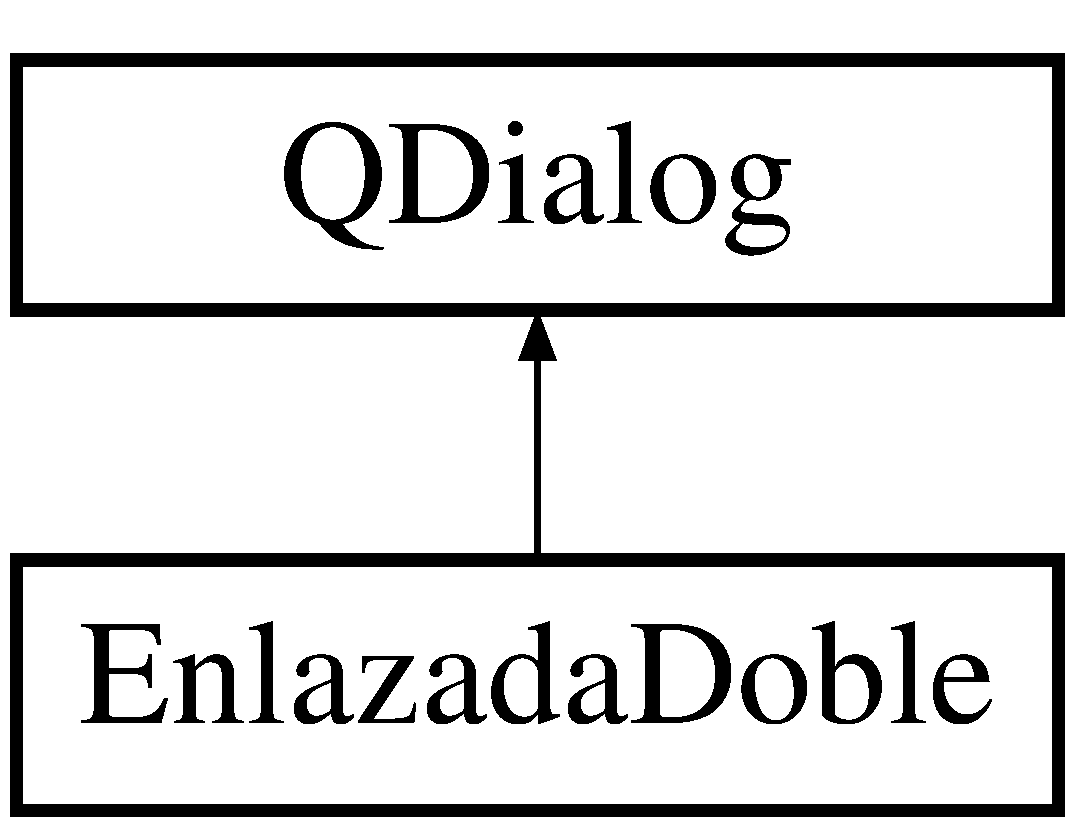
\includegraphics[height=2.000000cm]{class_enlazada_doble}
\end{center}
\end{figure}
\subsection*{Métodos públicos}
\begin{DoxyCompactItemize}
\item 
\mbox{\hyperlink{class_enlazada_doble_a5b55fdc97b66257ed864966d19a27439}{Enlazada\+Doble}} (Q\+Widget $\ast$parent=0)
\item 
\mbox{\hyperlink{class_enlazada_doble_a570a769129249be3c786e6ac21253bb8}{$\sim$\+Enlazada\+Doble}} ()
\end{DoxyCompactItemize}
\subsection*{Atributos públicos}
\begin{DoxyCompactItemize}
\item 
\mbox{\hyperlink{class_doble_linked_list}{Doble\+Linked\+List}} $\ast$ \mbox{\hyperlink{class_enlazada_doble_a041d141e37c6efade1cae5ea9f5d982c}{lista}}
\item 
int \mbox{\hyperlink{class_enlazada_doble_ac4cff0c052eef87b0211923a625daa4d}{posx}}
\end{DoxyCompactItemize}


\subsection{Descripción detallada}
The \mbox{\hyperlink{class_enlazada_doble}{Enlazada\+Doble}} class clase que contiene lo referente a la ventana de la lista doblemente enlazada. 

\subsection{Documentación del constructor y destructor}
\mbox{\Hypertarget{class_enlazada_doble_a5b55fdc97b66257ed864966d19a27439}\label{class_enlazada_doble_a5b55fdc97b66257ed864966d19a27439}} 
\index{Enlazada\+Doble@{Enlazada\+Doble}!Enlazada\+Doble@{Enlazada\+Doble}}
\index{Enlazada\+Doble@{Enlazada\+Doble}!Enlazada\+Doble@{Enlazada\+Doble}}
\subsubsection{\texorpdfstring{Enlazada\+Doble()}{EnlazadaDoble()}}
{\footnotesize\ttfamily Enlazada\+Doble\+::\+Enlazada\+Doble (\begin{DoxyParamCaption}\item[{Q\+Widget $\ast$}]{parent = {\ttfamily 0} }\end{DoxyParamCaption})\hspace{0.3cm}{\ttfamily [explicit]}}

\mbox{\Hypertarget{class_enlazada_doble_a570a769129249be3c786e6ac21253bb8}\label{class_enlazada_doble_a570a769129249be3c786e6ac21253bb8}} 
\index{Enlazada\+Doble@{Enlazada\+Doble}!````~Enlazada\+Doble@{$\sim$\+Enlazada\+Doble}}
\index{````~Enlazada\+Doble@{$\sim$\+Enlazada\+Doble}!Enlazada\+Doble@{Enlazada\+Doble}}
\subsubsection{\texorpdfstring{$\sim$\+Enlazada\+Doble()}{~EnlazadaDoble()}}
{\footnotesize\ttfamily Enlazada\+Doble\+::$\sim$\+Enlazada\+Doble (\begin{DoxyParamCaption}{ }\end{DoxyParamCaption})}



\subsection{Documentación de los datos miembro}
\mbox{\Hypertarget{class_enlazada_doble_a041d141e37c6efade1cae5ea9f5d982c}\label{class_enlazada_doble_a041d141e37c6efade1cae5ea9f5d982c}} 
\index{Enlazada\+Doble@{Enlazada\+Doble}!lista@{lista}}
\index{lista@{lista}!Enlazada\+Doble@{Enlazada\+Doble}}
\subsubsection{\texorpdfstring{lista}{lista}}
{\footnotesize\ttfamily \mbox{\hyperlink{class_doble_linked_list}{Doble\+Linked\+List}}$\ast$ Enlazada\+Doble\+::lista}

\mbox{\Hypertarget{class_enlazada_doble_ac4cff0c052eef87b0211923a625daa4d}\label{class_enlazada_doble_ac4cff0c052eef87b0211923a625daa4d}} 
\index{Enlazada\+Doble@{Enlazada\+Doble}!posx@{posx}}
\index{posx@{posx}!Enlazada\+Doble@{Enlazada\+Doble}}
\subsubsection{\texorpdfstring{posx}{posx}}
{\footnotesize\ttfamily int Enlazada\+Doble\+::posx}



La documentación para esta clase fue generada a partir de los siguientes ficheros\+:\begin{DoxyCompactItemize}
\item 
\mbox{\hyperlink{enlazadadoble_8h}{enlazadadoble.\+h}}\item 
\mbox{\hyperlink{enlazadadoble_8cpp}{enlazadadoble.\+cpp}}\end{DoxyCompactItemize}

\hypertarget{class_lista_simple}{}\section{Referencia de la Clase Lista\+Simple}
\label{class_lista_simple}\index{Lista\+Simple@{Lista\+Simple}}


The \mbox{\hyperlink{class_lista_simple}{Lista\+Simple}} class clase que contiene lo referente a la ventana de la lista simple.  




{\ttfamily \#include $<$listasimple.\+h$>$}

Diagrama de herencias de Lista\+Simple\begin{figure}[H]
\begin{center}
\leavevmode
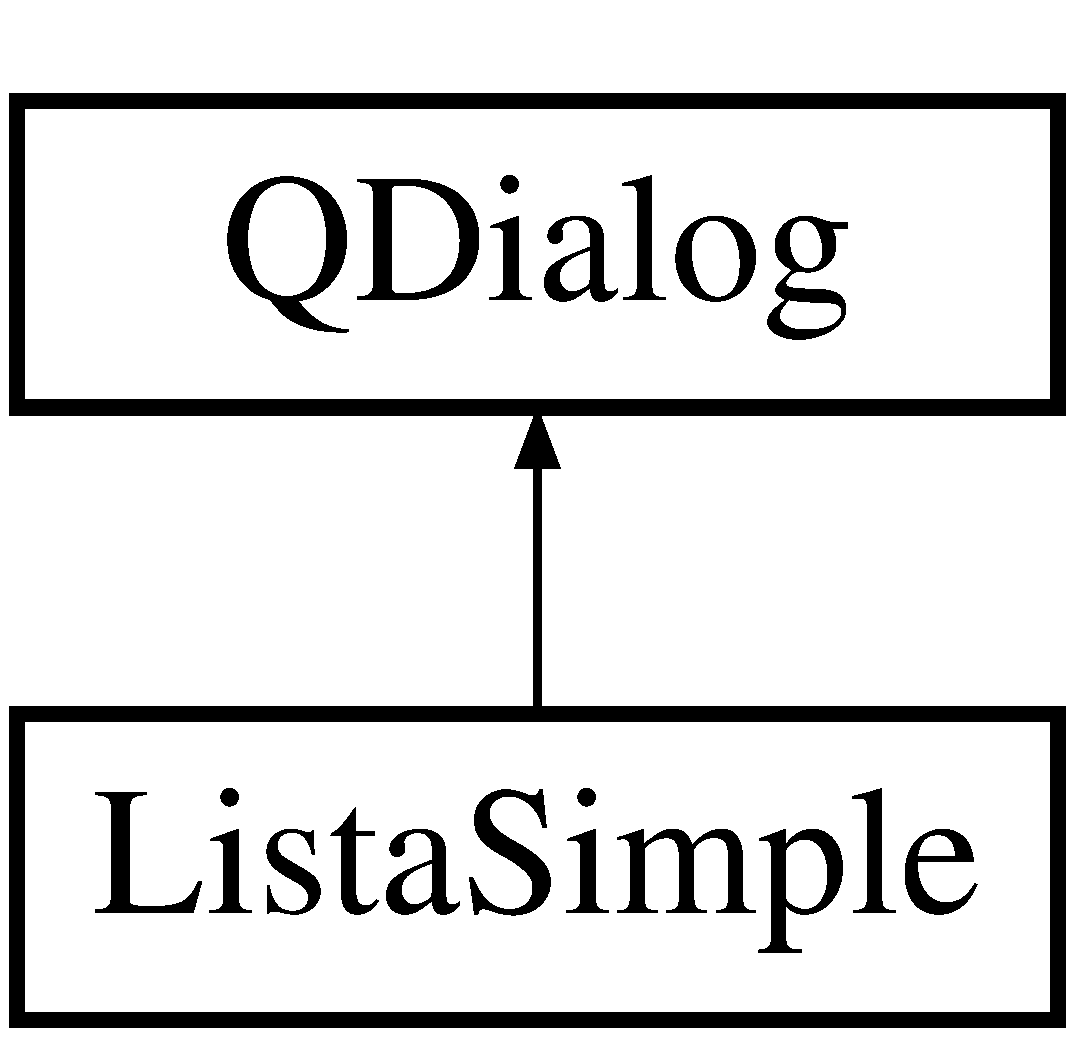
\includegraphics[height=2.000000cm]{class_lista_simple}
\end{center}
\end{figure}
\subsection*{Métodos públicos}
\begin{DoxyCompactItemize}
\item 
\mbox{\hyperlink{class_lista_simple_a8fd950a3f4bc90c23a163e9e381081f4}{Lista\+Simple}} (Q\+Widget $\ast$parent=0)
\item 
\mbox{\hyperlink{class_lista_simple_a44b1edd7d0e73b6e80748c712715e42a}{$\sim$\+Lista\+Simple}} ()
\end{DoxyCompactItemize}
\subsection*{Atributos públicos}
\begin{DoxyCompactItemize}
\item 
\mbox{\hyperlink{class_simple_linked_list}{Simple\+Linked\+List}} $\ast$ \mbox{\hyperlink{class_lista_simple_a46e5f8b712f9569021b223e60acabdaa}{lista}}
\item 
int \mbox{\hyperlink{class_lista_simple_a287deeb5d9e391d810d309798e8bf026}{posx}}
\end{DoxyCompactItemize}


\subsection{Descripción detallada}
The \mbox{\hyperlink{class_lista_simple}{Lista\+Simple}} class clase que contiene lo referente a la ventana de la lista simple. 

\subsection{Documentación del constructor y destructor}
\mbox{\Hypertarget{class_lista_simple_a8fd950a3f4bc90c23a163e9e381081f4}\label{class_lista_simple_a8fd950a3f4bc90c23a163e9e381081f4}} 
\index{Lista\+Simple@{Lista\+Simple}!Lista\+Simple@{Lista\+Simple}}
\index{Lista\+Simple@{Lista\+Simple}!Lista\+Simple@{Lista\+Simple}}
\subsubsection{\texorpdfstring{Lista\+Simple()}{ListaSimple()}}
{\footnotesize\ttfamily Lista\+Simple\+::\+Lista\+Simple (\begin{DoxyParamCaption}\item[{Q\+Widget $\ast$}]{parent = {\ttfamily 0} }\end{DoxyParamCaption})\hspace{0.3cm}{\ttfamily [explicit]}}

\mbox{\Hypertarget{class_lista_simple_a44b1edd7d0e73b6e80748c712715e42a}\label{class_lista_simple_a44b1edd7d0e73b6e80748c712715e42a}} 
\index{Lista\+Simple@{Lista\+Simple}!````~Lista\+Simple@{$\sim$\+Lista\+Simple}}
\index{````~Lista\+Simple@{$\sim$\+Lista\+Simple}!Lista\+Simple@{Lista\+Simple}}
\subsubsection{\texorpdfstring{$\sim$\+Lista\+Simple()}{~ListaSimple()}}
{\footnotesize\ttfamily Lista\+Simple\+::$\sim$\+Lista\+Simple (\begin{DoxyParamCaption}{ }\end{DoxyParamCaption})}



\subsection{Documentación de los datos miembro}
\mbox{\Hypertarget{class_lista_simple_a46e5f8b712f9569021b223e60acabdaa}\label{class_lista_simple_a46e5f8b712f9569021b223e60acabdaa}} 
\index{Lista\+Simple@{Lista\+Simple}!lista@{lista}}
\index{lista@{lista}!Lista\+Simple@{Lista\+Simple}}
\subsubsection{\texorpdfstring{lista}{lista}}
{\footnotesize\ttfamily \mbox{\hyperlink{class_simple_linked_list}{Simple\+Linked\+List}}$\ast$ Lista\+Simple\+::lista}

\mbox{\Hypertarget{class_lista_simple_a287deeb5d9e391d810d309798e8bf026}\label{class_lista_simple_a287deeb5d9e391d810d309798e8bf026}} 
\index{Lista\+Simple@{Lista\+Simple}!posx@{posx}}
\index{posx@{posx}!Lista\+Simple@{Lista\+Simple}}
\subsubsection{\texorpdfstring{posx}{posx}}
{\footnotesize\ttfamily int Lista\+Simple\+::posx}



La documentación para esta clase fue generada a partir de los siguientes ficheros\+:\begin{DoxyCompactItemize}
\item 
\mbox{\hyperlink{listasimple_8h}{listasimple.\+h}}\item 
\mbox{\hyperlink{listasimple_8cpp}{listasimple.\+cpp}}\end{DoxyCompactItemize}

\hypertarget{class_main_window}{}\section{Referencia de la Clase Main\+Window}
\label{class_main_window}\index{Main\+Window@{Main\+Window}}


The \mbox{\hyperlink{class_main_window}{Main\+Window}} class Esta clase controla todo lo referente a lo que se encuentra en la ventana inicial.  




{\ttfamily \#include $<$mainwindow.\+h$>$}

Diagrama de herencias de Main\+Window\begin{figure}[H]
\begin{center}
\leavevmode
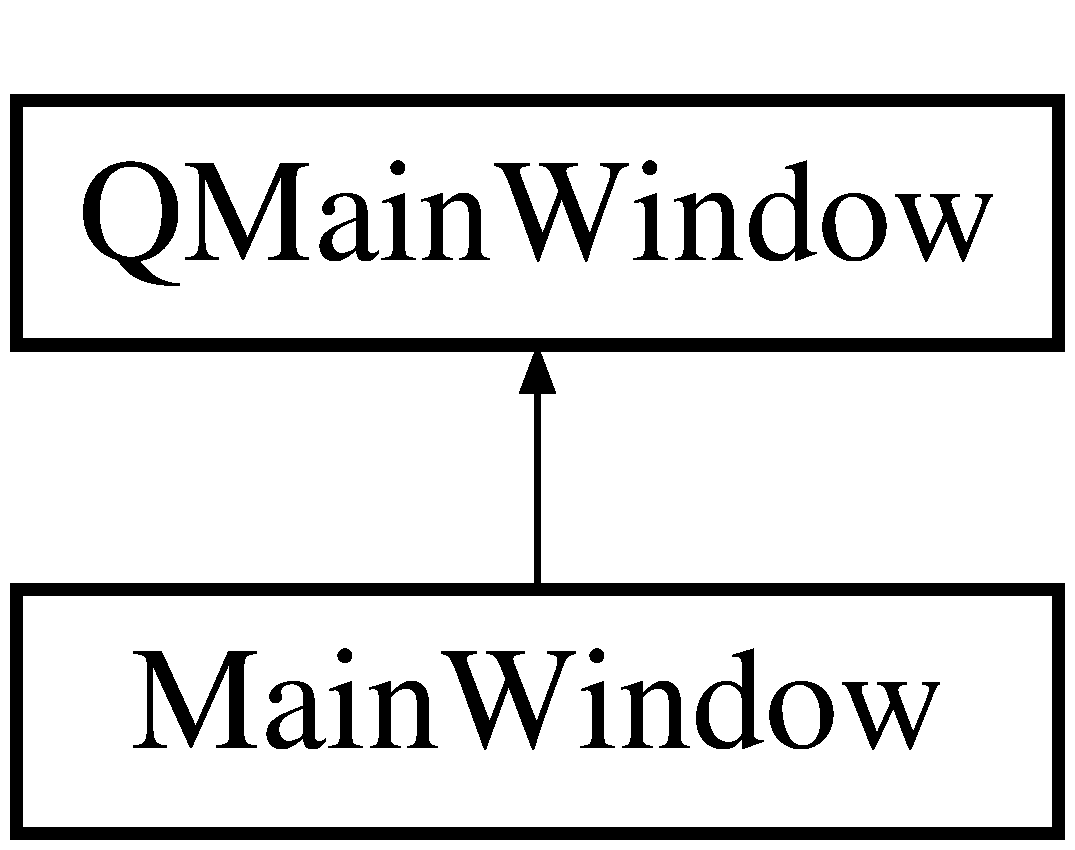
\includegraphics[height=2.000000cm]{class_main_window}
\end{center}
\end{figure}
\subsection*{Métodos públicos}
\begin{DoxyCompactItemize}
\item 
\mbox{\hyperlink{class_main_window_a8b244be8b7b7db1b08de2a2acb9409db}{Main\+Window}} (Q\+Widget $\ast$parent=0)
\item 
\mbox{\hyperlink{class_main_window_ae98d00a93bc118200eeef9f9bba1dba7}{$\sim$\+Main\+Window}} ()
\end{DoxyCompactItemize}


\subsection{Descripción detallada}
The \mbox{\hyperlink{class_main_window}{Main\+Window}} class Esta clase controla todo lo referente a lo que se encuentra en la ventana inicial. 

\subsection{Documentación del constructor y destructor}
\mbox{\Hypertarget{class_main_window_a8b244be8b7b7db1b08de2a2acb9409db}\label{class_main_window_a8b244be8b7b7db1b08de2a2acb9409db}} 
\index{Main\+Window@{Main\+Window}!Main\+Window@{Main\+Window}}
\index{Main\+Window@{Main\+Window}!Main\+Window@{Main\+Window}}
\subsubsection{\texorpdfstring{Main\+Window()}{MainWindow()}}
{\footnotesize\ttfamily Main\+Window\+::\+Main\+Window (\begin{DoxyParamCaption}\item[{Q\+Widget $\ast$}]{parent = {\ttfamily 0} }\end{DoxyParamCaption})\hspace{0.3cm}{\ttfamily [explicit]}}

\mbox{\Hypertarget{class_main_window_ae98d00a93bc118200eeef9f9bba1dba7}\label{class_main_window_ae98d00a93bc118200eeef9f9bba1dba7}} 
\index{Main\+Window@{Main\+Window}!````~Main\+Window@{$\sim$\+Main\+Window}}
\index{````~Main\+Window@{$\sim$\+Main\+Window}!Main\+Window@{Main\+Window}}
\subsubsection{\texorpdfstring{$\sim$\+Main\+Window()}{~MainWindow()}}
{\footnotesize\ttfamily Main\+Window\+::$\sim$\+Main\+Window (\begin{DoxyParamCaption}{ }\end{DoxyParamCaption})}



La documentación para esta clase fue generada a partir de los siguientes ficheros\+:\begin{DoxyCompactItemize}
\item 
\mbox{\hyperlink{mainwindow_8h}{mainwindow.\+h}}\item 
\mbox{\hyperlink{mainwindow_8cpp}{mainwindow.\+cpp}}\end{DoxyCompactItemize}

\hypertarget{class_nodo_doble_enlazado}{}\section{Referencia de la Clase Nodo\+Doble\+Enlazado}
\label{class_nodo_doble_enlazado}\index{Nodo\+Doble\+Enlazado@{Nodo\+Doble\+Enlazado}}


The \mbox{\hyperlink{class_nodo_doble_enlazado}{Nodo\+Doble\+Enlazado}} class Estructura de datos nodo para lista doble enlazada.  




{\ttfamily \#include $<$nododobleenlazado.\+h$>$}

\subsection*{Métodos públicos}
\begin{DoxyCompactItemize}
\item 
\mbox{\hyperlink{class_nodo_doble_enlazado_af8def34f6a5d897ae96434eabfbadd1d}{Nodo\+Doble\+Enlazado}} (Q\+String dat)
\begin{DoxyCompactList}\small\item\em \mbox{\hyperlink{class_nodo_doble_enlazado}{Nodo\+Doble\+Enlazado}} inicializa el nodo. \end{DoxyCompactList}\item 
Q\+String \mbox{\hyperlink{class_nodo_doble_enlazado_a2c464eb4789b8ad28891a308b6f52616}{get\+Dato}} ()
\begin{DoxyCompactList}\small\item\em get\+Dato retorna el dato que contiene el nodo \end{DoxyCompactList}\item 
void \mbox{\hyperlink{class_nodo_doble_enlazado_ae8fa0f3b992875c1031e49eabba670a8}{set\+Pos}} (int pos)
\begin{DoxyCompactList}\small\item\em set\+Pos establece la posicion en la lista del nodo \end{DoxyCompactList}\item 
int \mbox{\hyperlink{class_nodo_doble_enlazado_a73808d8a3ae1ca8094a5e6f0670277ca}{get\+Pos}} ()
\begin{DoxyCompactList}\small\item\em get\+Pos da la posicion del nodo \end{DoxyCompactList}\item 
void \mbox{\hyperlink{class_nodo_doble_enlazado_a7fe3c0a57d300f948bf1228da964a673}{set\+Dato}} (Q\+String dat)
\begin{DoxyCompactList}\small\item\em set\+Dato establece el dato del nodo \end{DoxyCompactList}\end{DoxyCompactItemize}
\subsection*{Atributos públicos}
\begin{DoxyCompactItemize}
\item 
\mbox{\hyperlink{class_nodo_doble_enlazado}{Nodo\+Doble\+Enlazado}} $\ast$ \mbox{\hyperlink{class_nodo_doble_enlazado_a5e67691aee2e78dd7d89f7df80ca84da}{siguiente}}
\item 
\mbox{\hyperlink{class_nodo_doble_enlazado}{Nodo\+Doble\+Enlazado}} $\ast$ \mbox{\hyperlink{class_nodo_doble_enlazado_aec27165ad44ca05a20a4c80f93db9c96}{anterior}}
\end{DoxyCompactItemize}


\subsection{Descripción detallada}
The \mbox{\hyperlink{class_nodo_doble_enlazado}{Nodo\+Doble\+Enlazado}} class Estructura de datos nodo para lista doble enlazada. 

\subsection{Documentación del constructor y destructor}
\mbox{\Hypertarget{class_nodo_doble_enlazado_af8def34f6a5d897ae96434eabfbadd1d}\label{class_nodo_doble_enlazado_af8def34f6a5d897ae96434eabfbadd1d}} 
\index{Nodo\+Doble\+Enlazado@{Nodo\+Doble\+Enlazado}!Nodo\+Doble\+Enlazado@{Nodo\+Doble\+Enlazado}}
\index{Nodo\+Doble\+Enlazado@{Nodo\+Doble\+Enlazado}!Nodo\+Doble\+Enlazado@{Nodo\+Doble\+Enlazado}}
\subsubsection{\texorpdfstring{Nodo\+Doble\+Enlazado()}{NodoDobleEnlazado()}}
{\footnotesize\ttfamily Nodo\+Doble\+Enlazado\+::\+Nodo\+Doble\+Enlazado (\begin{DoxyParamCaption}\item[{Q\+String}]{dat }\end{DoxyParamCaption})\hspace{0.3cm}{\ttfamily [inline]}}



\mbox{\hyperlink{class_nodo_doble_enlazado}{Nodo\+Doble\+Enlazado}} inicializa el nodo. 


\begin{DoxyParams}{Parámetros}
{\em dat} & dato del nodo \\
\hline
\end{DoxyParams}


\subsection{Documentación de las funciones miembro}
\mbox{\Hypertarget{class_nodo_doble_enlazado_a2c464eb4789b8ad28891a308b6f52616}\label{class_nodo_doble_enlazado_a2c464eb4789b8ad28891a308b6f52616}} 
\index{Nodo\+Doble\+Enlazado@{Nodo\+Doble\+Enlazado}!get\+Dato@{get\+Dato}}
\index{get\+Dato@{get\+Dato}!Nodo\+Doble\+Enlazado@{Nodo\+Doble\+Enlazado}}
\subsubsection{\texorpdfstring{get\+Dato()}{getDato()}}
{\footnotesize\ttfamily Q\+String Nodo\+Doble\+Enlazado\+::get\+Dato (\begin{DoxyParamCaption}{ }\end{DoxyParamCaption})\hspace{0.3cm}{\ttfamily [inline]}}



get\+Dato retorna el dato que contiene el nodo 

\begin{DoxyReturn}{Devuelve}
Q\+String del nodo 
\end{DoxyReturn}
\mbox{\Hypertarget{class_nodo_doble_enlazado_a73808d8a3ae1ca8094a5e6f0670277ca}\label{class_nodo_doble_enlazado_a73808d8a3ae1ca8094a5e6f0670277ca}} 
\index{Nodo\+Doble\+Enlazado@{Nodo\+Doble\+Enlazado}!get\+Pos@{get\+Pos}}
\index{get\+Pos@{get\+Pos}!Nodo\+Doble\+Enlazado@{Nodo\+Doble\+Enlazado}}
\subsubsection{\texorpdfstring{get\+Pos()}{getPos()}}
{\footnotesize\ttfamily int Nodo\+Doble\+Enlazado\+::get\+Pos (\begin{DoxyParamCaption}{ }\end{DoxyParamCaption})\hspace{0.3cm}{\ttfamily [inline]}}



get\+Pos da la posicion del nodo 

\begin{DoxyReturn}{Devuelve}
posicion del nodo 
\end{DoxyReturn}
\mbox{\Hypertarget{class_nodo_doble_enlazado_a7fe3c0a57d300f948bf1228da964a673}\label{class_nodo_doble_enlazado_a7fe3c0a57d300f948bf1228da964a673}} 
\index{Nodo\+Doble\+Enlazado@{Nodo\+Doble\+Enlazado}!set\+Dato@{set\+Dato}}
\index{set\+Dato@{set\+Dato}!Nodo\+Doble\+Enlazado@{Nodo\+Doble\+Enlazado}}
\subsubsection{\texorpdfstring{set\+Dato()}{setDato()}}
{\footnotesize\ttfamily void Nodo\+Doble\+Enlazado\+::set\+Dato (\begin{DoxyParamCaption}\item[{Q\+String}]{dat }\end{DoxyParamCaption})\hspace{0.3cm}{\ttfamily [inline]}}



set\+Dato establece el dato del nodo 


\begin{DoxyParams}{Parámetros}
{\em dat} & dato del nodo \\
\hline
\end{DoxyParams}
\mbox{\Hypertarget{class_nodo_doble_enlazado_ae8fa0f3b992875c1031e49eabba670a8}\label{class_nodo_doble_enlazado_ae8fa0f3b992875c1031e49eabba670a8}} 
\index{Nodo\+Doble\+Enlazado@{Nodo\+Doble\+Enlazado}!set\+Pos@{set\+Pos}}
\index{set\+Pos@{set\+Pos}!Nodo\+Doble\+Enlazado@{Nodo\+Doble\+Enlazado}}
\subsubsection{\texorpdfstring{set\+Pos()}{setPos()}}
{\footnotesize\ttfamily void Nodo\+Doble\+Enlazado\+::set\+Pos (\begin{DoxyParamCaption}\item[{int}]{pos }\end{DoxyParamCaption})\hspace{0.3cm}{\ttfamily [inline]}}



set\+Pos establece la posicion en la lista del nodo 


\begin{DoxyParams}{Parámetros}
{\em pos} & entero de la posicion \\
\hline
\end{DoxyParams}


\subsection{Documentación de los datos miembro}
\mbox{\Hypertarget{class_nodo_doble_enlazado_aec27165ad44ca05a20a4c80f93db9c96}\label{class_nodo_doble_enlazado_aec27165ad44ca05a20a4c80f93db9c96}} 
\index{Nodo\+Doble\+Enlazado@{Nodo\+Doble\+Enlazado}!anterior@{anterior}}
\index{anterior@{anterior}!Nodo\+Doble\+Enlazado@{Nodo\+Doble\+Enlazado}}
\subsubsection{\texorpdfstring{anterior}{anterior}}
{\footnotesize\ttfamily \mbox{\hyperlink{class_nodo_doble_enlazado}{Nodo\+Doble\+Enlazado}}$\ast$ Nodo\+Doble\+Enlazado\+::anterior}

\mbox{\Hypertarget{class_nodo_doble_enlazado_a5e67691aee2e78dd7d89f7df80ca84da}\label{class_nodo_doble_enlazado_a5e67691aee2e78dd7d89f7df80ca84da}} 
\index{Nodo\+Doble\+Enlazado@{Nodo\+Doble\+Enlazado}!siguiente@{siguiente}}
\index{siguiente@{siguiente}!Nodo\+Doble\+Enlazado@{Nodo\+Doble\+Enlazado}}
\subsubsection{\texorpdfstring{siguiente}{siguiente}}
{\footnotesize\ttfamily \mbox{\hyperlink{class_nodo_doble_enlazado}{Nodo\+Doble\+Enlazado}}$\ast$ Nodo\+Doble\+Enlazado\+::siguiente}



La documentación para esta clase fue generada a partir del siguiente fichero\+:\begin{DoxyCompactItemize}
\item 
\mbox{\hyperlink{nododobleenlazado_8h}{nododobleenlazado.\+h}}\end{DoxyCompactItemize}

\hypertarget{class_nodo_lista_circular}{}\section{Referencia de la Clase Nodo\+Lista\+Circular}
\label{class_nodo_lista_circular}\index{Nodo\+Lista\+Circular@{Nodo\+Lista\+Circular}}


The \mbox{\hyperlink{class_nodo_lista_circular}{Nodo\+Lista\+Circular}} class Estructura del nodo de la lista circular.  




{\ttfamily \#include $<$nodolistacircular.\+h$>$}

\subsection*{Métodos públicos}
\begin{DoxyCompactItemize}
\item 
\mbox{\hyperlink{class_nodo_lista_circular_a545fa0b7acf627390514fe87b6aff277}{Nodo\+Lista\+Circular}} (Q\+String dat)
\begin{DoxyCompactList}\small\item\em \mbox{\hyperlink{class_nodo_lista_circular}{Nodo\+Lista\+Circular}} inicializa el nodo. \end{DoxyCompactList}\item 
Q\+String \mbox{\hyperlink{class_nodo_lista_circular_a37393a1f2c117891206678387d2a9837}{get\+Dato}} ()
\begin{DoxyCompactList}\small\item\em get\+Dato da el dato que contiene el nodo \end{DoxyCompactList}\item 
void \mbox{\hyperlink{class_nodo_lista_circular_aa6307fda1bf33f2d8035893ee9fea81a}{set\+Pos}} (int pos)
\begin{DoxyCompactList}\small\item\em set\+Pos establece la posicion del nodo \end{DoxyCompactList}\item 
int \mbox{\hyperlink{class_nodo_lista_circular_a5e835714bbc78795e50e6c76a3157ff4}{get\+Pos}} ()
\begin{DoxyCompactList}\small\item\em get\+Pos da la posicon del nodo \end{DoxyCompactList}\item 
void \mbox{\hyperlink{class_nodo_lista_circular_a3f2bd335e477f76dfcb2417686ca6296}{set\+Dato}} (Q\+String dat)
\begin{DoxyCompactList}\small\item\em set\+Dato establece el dato del nodo \end{DoxyCompactList}\end{DoxyCompactItemize}
\subsection*{Atributos públicos}
\begin{DoxyCompactItemize}
\item 
\mbox{\hyperlink{class_nodo_lista_circular}{Nodo\+Lista\+Circular}} $\ast$ \mbox{\hyperlink{class_nodo_lista_circular_a689ddba0f9da231ef3bfdcd4a0d45ae3}{siguiente}}
\item 
\mbox{\hyperlink{class_nodo_lista_circular}{Nodo\+Lista\+Circular}} $\ast$ \mbox{\hyperlink{class_nodo_lista_circular_a62c97352f8df5d9b817568467d90ee33}{anterior}}
\end{DoxyCompactItemize}


\subsection{Descripción detallada}
The \mbox{\hyperlink{class_nodo_lista_circular}{Nodo\+Lista\+Circular}} class Estructura del nodo de la lista circular. 

\subsection{Documentación del constructor y destructor}
\mbox{\Hypertarget{class_nodo_lista_circular_a545fa0b7acf627390514fe87b6aff277}\label{class_nodo_lista_circular_a545fa0b7acf627390514fe87b6aff277}} 
\index{Nodo\+Lista\+Circular@{Nodo\+Lista\+Circular}!Nodo\+Lista\+Circular@{Nodo\+Lista\+Circular}}
\index{Nodo\+Lista\+Circular@{Nodo\+Lista\+Circular}!Nodo\+Lista\+Circular@{Nodo\+Lista\+Circular}}
\subsubsection{\texorpdfstring{Nodo\+Lista\+Circular()}{NodoListaCircular()}}
{\footnotesize\ttfamily Nodo\+Lista\+Circular\+::\+Nodo\+Lista\+Circular (\begin{DoxyParamCaption}\item[{Q\+String}]{dat }\end{DoxyParamCaption})\hspace{0.3cm}{\ttfamily [inline]}}



\mbox{\hyperlink{class_nodo_lista_circular}{Nodo\+Lista\+Circular}} inicializa el nodo. 


\begin{DoxyParams}{Parámetros}
{\em dat} & dato que va a contener el nodo \\
\hline
\end{DoxyParams}


\subsection{Documentación de las funciones miembro}
\mbox{\Hypertarget{class_nodo_lista_circular_a37393a1f2c117891206678387d2a9837}\label{class_nodo_lista_circular_a37393a1f2c117891206678387d2a9837}} 
\index{Nodo\+Lista\+Circular@{Nodo\+Lista\+Circular}!get\+Dato@{get\+Dato}}
\index{get\+Dato@{get\+Dato}!Nodo\+Lista\+Circular@{Nodo\+Lista\+Circular}}
\subsubsection{\texorpdfstring{get\+Dato()}{getDato()}}
{\footnotesize\ttfamily Q\+String Nodo\+Lista\+Circular\+::get\+Dato (\begin{DoxyParamCaption}{ }\end{DoxyParamCaption})\hspace{0.3cm}{\ttfamily [inline]}}



get\+Dato da el dato que contiene el nodo 

\begin{DoxyReturn}{Devuelve}
dato del nodo 
\end{DoxyReturn}
\mbox{\Hypertarget{class_nodo_lista_circular_a5e835714bbc78795e50e6c76a3157ff4}\label{class_nodo_lista_circular_a5e835714bbc78795e50e6c76a3157ff4}} 
\index{Nodo\+Lista\+Circular@{Nodo\+Lista\+Circular}!get\+Pos@{get\+Pos}}
\index{get\+Pos@{get\+Pos}!Nodo\+Lista\+Circular@{Nodo\+Lista\+Circular}}
\subsubsection{\texorpdfstring{get\+Pos()}{getPos()}}
{\footnotesize\ttfamily int Nodo\+Lista\+Circular\+::get\+Pos (\begin{DoxyParamCaption}{ }\end{DoxyParamCaption})\hspace{0.3cm}{\ttfamily [inline]}}



get\+Pos da la posicon del nodo 

\begin{DoxyReturn}{Devuelve}
entero de la posicion 
\end{DoxyReturn}
\mbox{\Hypertarget{class_nodo_lista_circular_a3f2bd335e477f76dfcb2417686ca6296}\label{class_nodo_lista_circular_a3f2bd335e477f76dfcb2417686ca6296}} 
\index{Nodo\+Lista\+Circular@{Nodo\+Lista\+Circular}!set\+Dato@{set\+Dato}}
\index{set\+Dato@{set\+Dato}!Nodo\+Lista\+Circular@{Nodo\+Lista\+Circular}}
\subsubsection{\texorpdfstring{set\+Dato()}{setDato()}}
{\footnotesize\ttfamily void Nodo\+Lista\+Circular\+::set\+Dato (\begin{DoxyParamCaption}\item[{Q\+String}]{dat }\end{DoxyParamCaption})\hspace{0.3cm}{\ttfamily [inline]}}



set\+Dato establece el dato del nodo 


\begin{DoxyParams}{Parámetros}
{\em dat} & dato del nodo \\
\hline
\end{DoxyParams}
\mbox{\Hypertarget{class_nodo_lista_circular_aa6307fda1bf33f2d8035893ee9fea81a}\label{class_nodo_lista_circular_aa6307fda1bf33f2d8035893ee9fea81a}} 
\index{Nodo\+Lista\+Circular@{Nodo\+Lista\+Circular}!set\+Pos@{set\+Pos}}
\index{set\+Pos@{set\+Pos}!Nodo\+Lista\+Circular@{Nodo\+Lista\+Circular}}
\subsubsection{\texorpdfstring{set\+Pos()}{setPos()}}
{\footnotesize\ttfamily void Nodo\+Lista\+Circular\+::set\+Pos (\begin{DoxyParamCaption}\item[{int}]{pos }\end{DoxyParamCaption})\hspace{0.3cm}{\ttfamily [inline]}}



set\+Pos establece la posicion del nodo 


\begin{DoxyParams}{Parámetros}
{\em pos} & posicion del nodo \\
\hline
\end{DoxyParams}


\subsection{Documentación de los datos miembro}
\mbox{\Hypertarget{class_nodo_lista_circular_a62c97352f8df5d9b817568467d90ee33}\label{class_nodo_lista_circular_a62c97352f8df5d9b817568467d90ee33}} 
\index{Nodo\+Lista\+Circular@{Nodo\+Lista\+Circular}!anterior@{anterior}}
\index{anterior@{anterior}!Nodo\+Lista\+Circular@{Nodo\+Lista\+Circular}}
\subsubsection{\texorpdfstring{anterior}{anterior}}
{\footnotesize\ttfamily \mbox{\hyperlink{class_nodo_lista_circular}{Nodo\+Lista\+Circular}}$\ast$ Nodo\+Lista\+Circular\+::anterior}

\mbox{\Hypertarget{class_nodo_lista_circular_a689ddba0f9da231ef3bfdcd4a0d45ae3}\label{class_nodo_lista_circular_a689ddba0f9da231ef3bfdcd4a0d45ae3}} 
\index{Nodo\+Lista\+Circular@{Nodo\+Lista\+Circular}!siguiente@{siguiente}}
\index{siguiente@{siguiente}!Nodo\+Lista\+Circular@{Nodo\+Lista\+Circular}}
\subsubsection{\texorpdfstring{siguiente}{siguiente}}
{\footnotesize\ttfamily \mbox{\hyperlink{class_nodo_lista_circular}{Nodo\+Lista\+Circular}}$\ast$ Nodo\+Lista\+Circular\+::siguiente}



La documentación para esta clase fue generada a partir del siguiente fichero\+:\begin{DoxyCompactItemize}
\item 
\mbox{\hyperlink{nodolistacircular_8h}{nodolistacircular.\+h}}\end{DoxyCompactItemize}

\hypertarget{class_nodo_simple}{}\section{Referencia de la Clase Nodo\+Simple}
\label{class_nodo_simple}\index{Nodo\+Simple@{Nodo\+Simple}}


The \mbox{\hyperlink{class_nodo_simple}{Nodo\+Simple}} class Estructura del nodo de la lista simple.  




{\ttfamily \#include $<$nodosimple.\+h$>$}

\subsection*{Métodos públicos}
\begin{DoxyCompactItemize}
\item 
\mbox{\hyperlink{class_nodo_simple_acde7a8d315007bd580fbff42eaa69c9c}{Nodo\+Simple}} (Q\+String dat)
\begin{DoxyCompactList}\small\item\em \mbox{\hyperlink{class_nodo_simple}{Nodo\+Simple}} incia el nodo. \end{DoxyCompactList}\item 
Q\+String \mbox{\hyperlink{class_nodo_simple_a8e2cf29c0b691d7c81a4a1f2c9414863}{get\+Dato}} ()
\begin{DoxyCompactList}\small\item\em get\+Dato da el dato del nodo \end{DoxyCompactList}\item 
void \mbox{\hyperlink{class_nodo_simple_a455c9a0f62ba752d4e29e54fd588cdd1}{set\+Pos}} (int pos)
\begin{DoxyCompactList}\small\item\em set\+Pos establece la posicion del nodo \end{DoxyCompactList}\item 
int \mbox{\hyperlink{class_nodo_simple_a6808405a250b6a7b097d34767dfa9b30}{get\+Pos}} ()
\begin{DoxyCompactList}\small\item\em get\+Pos da la posicion del nodo \end{DoxyCompactList}\item 
void \mbox{\hyperlink{class_nodo_simple_ab32eeae9ba44f0464a5d45c69602cd11}{set\+Dato}} (Q\+String dat)
\begin{DoxyCompactList}\small\item\em set\+Dato establece el dato del nodo \end{DoxyCompactList}\end{DoxyCompactItemize}
\subsection*{Atributos públicos}
\begin{DoxyCompactItemize}
\item 
\mbox{\hyperlink{class_nodo_simple}{Nodo\+Simple}} $\ast$ \mbox{\hyperlink{class_nodo_simple_a7ef0a1b5d9ee22ee78dfbf29e25e8450}{siguiente}}
\end{DoxyCompactItemize}


\subsection{Descripción detallada}
The \mbox{\hyperlink{class_nodo_simple}{Nodo\+Simple}} class Estructura del nodo de la lista simple. 

\subsection{Documentación del constructor y destructor}
\mbox{\Hypertarget{class_nodo_simple_acde7a8d315007bd580fbff42eaa69c9c}\label{class_nodo_simple_acde7a8d315007bd580fbff42eaa69c9c}} 
\index{Nodo\+Simple@{Nodo\+Simple}!Nodo\+Simple@{Nodo\+Simple}}
\index{Nodo\+Simple@{Nodo\+Simple}!Nodo\+Simple@{Nodo\+Simple}}
\subsubsection{\texorpdfstring{Nodo\+Simple()}{NodoSimple()}}
{\footnotesize\ttfamily Nodo\+Simple\+::\+Nodo\+Simple (\begin{DoxyParamCaption}\item[{Q\+String}]{dat }\end{DoxyParamCaption})\hspace{0.3cm}{\ttfamily [inline]}}



\mbox{\hyperlink{class_nodo_simple}{Nodo\+Simple}} incia el nodo. 


\begin{DoxyParams}{Parámetros}
{\em dat} & \\
\hline
\end{DoxyParams}


\subsection{Documentación de las funciones miembro}
\mbox{\Hypertarget{class_nodo_simple_a8e2cf29c0b691d7c81a4a1f2c9414863}\label{class_nodo_simple_a8e2cf29c0b691d7c81a4a1f2c9414863}} 
\index{Nodo\+Simple@{Nodo\+Simple}!get\+Dato@{get\+Dato}}
\index{get\+Dato@{get\+Dato}!Nodo\+Simple@{Nodo\+Simple}}
\subsubsection{\texorpdfstring{get\+Dato()}{getDato()}}
{\footnotesize\ttfamily Q\+String Nodo\+Simple\+::get\+Dato (\begin{DoxyParamCaption}{ }\end{DoxyParamCaption})\hspace{0.3cm}{\ttfamily [inline]}}



get\+Dato da el dato del nodo 

\begin{DoxyReturn}{Devuelve}
Q\+String del nodo 
\end{DoxyReturn}
\mbox{\Hypertarget{class_nodo_simple_a6808405a250b6a7b097d34767dfa9b30}\label{class_nodo_simple_a6808405a250b6a7b097d34767dfa9b30}} 
\index{Nodo\+Simple@{Nodo\+Simple}!get\+Pos@{get\+Pos}}
\index{get\+Pos@{get\+Pos}!Nodo\+Simple@{Nodo\+Simple}}
\subsubsection{\texorpdfstring{get\+Pos()}{getPos()}}
{\footnotesize\ttfamily int Nodo\+Simple\+::get\+Pos (\begin{DoxyParamCaption}{ }\end{DoxyParamCaption})\hspace{0.3cm}{\ttfamily [inline]}}



get\+Pos da la posicion del nodo 

\begin{DoxyReturn}{Devuelve}
entero con la posicion del nodo 
\end{DoxyReturn}
\mbox{\Hypertarget{class_nodo_simple_ab32eeae9ba44f0464a5d45c69602cd11}\label{class_nodo_simple_ab32eeae9ba44f0464a5d45c69602cd11}} 
\index{Nodo\+Simple@{Nodo\+Simple}!set\+Dato@{set\+Dato}}
\index{set\+Dato@{set\+Dato}!Nodo\+Simple@{Nodo\+Simple}}
\subsubsection{\texorpdfstring{set\+Dato()}{setDato()}}
{\footnotesize\ttfamily void Nodo\+Simple\+::set\+Dato (\begin{DoxyParamCaption}\item[{Q\+String}]{dat }\end{DoxyParamCaption})\hspace{0.3cm}{\ttfamily [inline]}}



set\+Dato establece el dato del nodo 


\begin{DoxyParams}{Parámetros}
{\em dat} & dato del nodo \\
\hline
\end{DoxyParams}
\mbox{\Hypertarget{class_nodo_simple_a455c9a0f62ba752d4e29e54fd588cdd1}\label{class_nodo_simple_a455c9a0f62ba752d4e29e54fd588cdd1}} 
\index{Nodo\+Simple@{Nodo\+Simple}!set\+Pos@{set\+Pos}}
\index{set\+Pos@{set\+Pos}!Nodo\+Simple@{Nodo\+Simple}}
\subsubsection{\texorpdfstring{set\+Pos()}{setPos()}}
{\footnotesize\ttfamily void Nodo\+Simple\+::set\+Pos (\begin{DoxyParamCaption}\item[{int}]{pos }\end{DoxyParamCaption})\hspace{0.3cm}{\ttfamily [inline]}}



set\+Pos establece la posicion del nodo 


\begin{DoxyParams}{Parámetros}
{\em pos} & posicion del nodo \\
\hline
\end{DoxyParams}


\subsection{Documentación de los datos miembro}
\mbox{\Hypertarget{class_nodo_simple_a7ef0a1b5d9ee22ee78dfbf29e25e8450}\label{class_nodo_simple_a7ef0a1b5d9ee22ee78dfbf29e25e8450}} 
\index{Nodo\+Simple@{Nodo\+Simple}!siguiente@{siguiente}}
\index{siguiente@{siguiente}!Nodo\+Simple@{Nodo\+Simple}}
\subsubsection{\texorpdfstring{siguiente}{siguiente}}
{\footnotesize\ttfamily \mbox{\hyperlink{class_nodo_simple}{Nodo\+Simple}}$\ast$ Nodo\+Simple\+::siguiente}



La documentación para esta clase fue generada a partir del siguiente fichero\+:\begin{DoxyCompactItemize}
\item 
\mbox{\hyperlink{nodosimple_8h}{nodosimple.\+h}}\end{DoxyCompactItemize}

\hypertarget{class_simple_linked_list}{}\section{Referencia de la Clase Simple\+Linked\+List}
\label{class_simple_linked_list}\index{Simple\+Linked\+List@{Simple\+Linked\+List}}


The \mbox{\hyperlink{class_simple_linked_list}{Simple\+Linked\+List}} class Estructura de la lista simple.  




{\ttfamily \#include $<$simplelinkedlist.\+h$>$}

\subsection*{Métodos públicos}
\begin{DoxyCompactItemize}
\item 
\mbox{\hyperlink{class_simple_linked_list_a508909ddc17e7be9e6c37554cac42bf7}{Simple\+Linked\+List}} ()
\begin{DoxyCompactList}\small\item\em \mbox{\hyperlink{class_simple_linked_list}{Simple\+Linked\+List}} incializa la lista simple. \end{DoxyCompactList}\item 
void \mbox{\hyperlink{class_simple_linked_list_aac2d1b432374ecbc20e8d9c5ba738fa7}{insertar\+Por\+Posicion}} (int pos, Q\+String dato)
\begin{DoxyCompactList}\small\item\em insertar\+Por\+Posicion inserta un nodo en una posicion en especifico \end{DoxyCompactList}\item 
void \mbox{\hyperlink{class_simple_linked_list_a2da267887f7b64579e3eb56c1940b20a}{ingresar\+Dato\+Final}} (Q\+String dato)
\begin{DoxyCompactList}\small\item\em ingresar\+Dato\+Final inserta un dato al final de la lista \end{DoxyCompactList}\item 
void \mbox{\hyperlink{class_simple_linked_list_aef2841b155c31147e5932c13302f39c4}{ingresar\+Dato\+Inicio}} (Q\+String dato)
\begin{DoxyCompactList}\small\item\em ingresar\+Dato\+Inicio inserta un nodo al inicio de la lista \end{DoxyCompactList}\item 
void \mbox{\hyperlink{class_simple_linked_list_a260b6de5d5c73652fa016c3b63222bae}{eliminar\+Posicion}} (int pos)
\begin{DoxyCompactList}\small\item\em eliminar\+Posicion elimina un nodo en una posicion en especifico \end{DoxyCompactList}\item 
void \mbox{\hyperlink{class_simple_linked_list_a398074e6af83b72302153bef22e5a899}{eliminar\+Inicio}} ()
\begin{DoxyCompactList}\small\item\em eliminar\+Inicio elimina el nodo del inicio de la lista \end{DoxyCompactList}\item 
void \mbox{\hyperlink{class_simple_linked_list_aabf382c8f9262f7b23718f60c1ef724d}{eliminar\+Final}} ()
\begin{DoxyCompactList}\small\item\em eliminar\+Final elimina el nodo del final de la lista \end{DoxyCompactList}\item 
void \mbox{\hyperlink{class_simple_linked_list_a4ad22b92d55951e72e45dcf7f2867a5d}{imprimir\+Lista}} ()
\begin{DoxyCompactList}\small\item\em imprimir\+Lista imprime la lista \end{DoxyCompactList}\item 
void \mbox{\hyperlink{class_simple_linked_list_ac2d7b784c2c5b20824a4ab54ce20eaa7}{editar}} (int pos, Q\+String dato)
\begin{DoxyCompactList}\small\item\em editar edita el dato de un nodo en especifico \end{DoxyCompactList}\item 
\mbox{\hyperlink{class_nodo_simple}{Nodo\+Simple}} \mbox{\hyperlink{class_simple_linked_list_a443815291e245287229b5aca1d963faf}{obtenerpor\+Posicion}} (int pos)
\begin{DoxyCompactList}\small\item\em obtenerpor\+Posicion retorna el nodo que se esta buscando \end{DoxyCompactList}\end{DoxyCompactItemize}
\subsection*{Atributos públicos}
\begin{DoxyCompactItemize}
\item 
\mbox{\hyperlink{class_nodo_simple}{Nodo\+Simple}} $\ast$ \mbox{\hyperlink{class_simple_linked_list_a8bfa0f48fc7ace062a1220477f7e824b}{primero}}
\item 
\mbox{\hyperlink{class_nodo_simple}{Nodo\+Simple}} $\ast$ \mbox{\hyperlink{class_simple_linked_list_a2f2e30e2a9c1a8bfdf518bc28b6fcf0c}{ultimo}}
\item 
int \mbox{\hyperlink{class_simple_linked_list_acb900363f7077cdb4036bef55a16671d}{largo}} = 0
\end{DoxyCompactItemize}


\subsection{Descripción detallada}
The \mbox{\hyperlink{class_simple_linked_list}{Simple\+Linked\+List}} class Estructura de la lista simple. 

\subsection{Documentación del constructor y destructor}
\mbox{\Hypertarget{class_simple_linked_list_a508909ddc17e7be9e6c37554cac42bf7}\label{class_simple_linked_list_a508909ddc17e7be9e6c37554cac42bf7}} 
\index{Simple\+Linked\+List@{Simple\+Linked\+List}!Simple\+Linked\+List@{Simple\+Linked\+List}}
\index{Simple\+Linked\+List@{Simple\+Linked\+List}!Simple\+Linked\+List@{Simple\+Linked\+List}}
\subsubsection{\texorpdfstring{Simple\+Linked\+List()}{SimpleLinkedList()}}
{\footnotesize\ttfamily Simple\+Linked\+List\+::\+Simple\+Linked\+List (\begin{DoxyParamCaption}{ }\end{DoxyParamCaption})\hspace{0.3cm}{\ttfamily [inline]}}



\mbox{\hyperlink{class_simple_linked_list}{Simple\+Linked\+List}} incializa la lista simple. 



\subsection{Documentación de las funciones miembro}
\mbox{\Hypertarget{class_simple_linked_list_ac2d7b784c2c5b20824a4ab54ce20eaa7}\label{class_simple_linked_list_ac2d7b784c2c5b20824a4ab54ce20eaa7}} 
\index{Simple\+Linked\+List@{Simple\+Linked\+List}!editar@{editar}}
\index{editar@{editar}!Simple\+Linked\+List@{Simple\+Linked\+List}}
\subsubsection{\texorpdfstring{editar()}{editar()}}
{\footnotesize\ttfamily void Simple\+Linked\+List\+::editar (\begin{DoxyParamCaption}\item[{int}]{pos,  }\item[{Q\+String}]{dato }\end{DoxyParamCaption})\hspace{0.3cm}{\ttfamily [inline]}}



editar edita el dato de un nodo en especifico 


\begin{DoxyParams}{Parámetros}
{\em pos} & posicion del nodo que se quiere editar \\
\hline
{\em dato} & dato por el que se quiere modificar \\
\hline
\end{DoxyParams}
\mbox{\Hypertarget{class_simple_linked_list_aabf382c8f9262f7b23718f60c1ef724d}\label{class_simple_linked_list_aabf382c8f9262f7b23718f60c1ef724d}} 
\index{Simple\+Linked\+List@{Simple\+Linked\+List}!eliminar\+Final@{eliminar\+Final}}
\index{eliminar\+Final@{eliminar\+Final}!Simple\+Linked\+List@{Simple\+Linked\+List}}
\subsubsection{\texorpdfstring{eliminar\+Final()}{eliminarFinal()}}
{\footnotesize\ttfamily void Simple\+Linked\+List\+::eliminar\+Final (\begin{DoxyParamCaption}{ }\end{DoxyParamCaption})\hspace{0.3cm}{\ttfamily [inline]}}



eliminar\+Final elimina el nodo del final de la lista 

\mbox{\Hypertarget{class_simple_linked_list_a398074e6af83b72302153bef22e5a899}\label{class_simple_linked_list_a398074e6af83b72302153bef22e5a899}} 
\index{Simple\+Linked\+List@{Simple\+Linked\+List}!eliminar\+Inicio@{eliminar\+Inicio}}
\index{eliminar\+Inicio@{eliminar\+Inicio}!Simple\+Linked\+List@{Simple\+Linked\+List}}
\subsubsection{\texorpdfstring{eliminar\+Inicio()}{eliminarInicio()}}
{\footnotesize\ttfamily void Simple\+Linked\+List\+::eliminar\+Inicio (\begin{DoxyParamCaption}{ }\end{DoxyParamCaption})\hspace{0.3cm}{\ttfamily [inline]}}



eliminar\+Inicio elimina el nodo del inicio de la lista 

\mbox{\Hypertarget{class_simple_linked_list_a260b6de5d5c73652fa016c3b63222bae}\label{class_simple_linked_list_a260b6de5d5c73652fa016c3b63222bae}} 
\index{Simple\+Linked\+List@{Simple\+Linked\+List}!eliminar\+Posicion@{eliminar\+Posicion}}
\index{eliminar\+Posicion@{eliminar\+Posicion}!Simple\+Linked\+List@{Simple\+Linked\+List}}
\subsubsection{\texorpdfstring{eliminar\+Posicion()}{eliminarPosicion()}}
{\footnotesize\ttfamily void Simple\+Linked\+List\+::eliminar\+Posicion (\begin{DoxyParamCaption}\item[{int}]{pos }\end{DoxyParamCaption})\hspace{0.3cm}{\ttfamily [inline]}}



eliminar\+Posicion elimina un nodo en una posicion en especifico 


\begin{DoxyParams}{Parámetros}
{\em pos} & posicion en la que se va a eliminar \\
\hline
\end{DoxyParams}
\mbox{\Hypertarget{class_simple_linked_list_a4ad22b92d55951e72e45dcf7f2867a5d}\label{class_simple_linked_list_a4ad22b92d55951e72e45dcf7f2867a5d}} 
\index{Simple\+Linked\+List@{Simple\+Linked\+List}!imprimir\+Lista@{imprimir\+Lista}}
\index{imprimir\+Lista@{imprimir\+Lista}!Simple\+Linked\+List@{Simple\+Linked\+List}}
\subsubsection{\texorpdfstring{imprimir\+Lista()}{imprimirLista()}}
{\footnotesize\ttfamily void Simple\+Linked\+List\+::imprimir\+Lista (\begin{DoxyParamCaption}{ }\end{DoxyParamCaption})\hspace{0.3cm}{\ttfamily [inline]}}



imprimir\+Lista imprime la lista 

\mbox{\Hypertarget{class_simple_linked_list_a2da267887f7b64579e3eb56c1940b20a}\label{class_simple_linked_list_a2da267887f7b64579e3eb56c1940b20a}} 
\index{Simple\+Linked\+List@{Simple\+Linked\+List}!ingresar\+Dato\+Final@{ingresar\+Dato\+Final}}
\index{ingresar\+Dato\+Final@{ingresar\+Dato\+Final}!Simple\+Linked\+List@{Simple\+Linked\+List}}
\subsubsection{\texorpdfstring{ingresar\+Dato\+Final()}{ingresarDatoFinal()}}
{\footnotesize\ttfamily void Simple\+Linked\+List\+::ingresar\+Dato\+Final (\begin{DoxyParamCaption}\item[{Q\+String}]{dato }\end{DoxyParamCaption})\hspace{0.3cm}{\ttfamily [inline]}}



ingresar\+Dato\+Final inserta un dato al final de la lista 


\begin{DoxyParams}{Parámetros}
{\em dato} & dato del nodo \\
\hline
\end{DoxyParams}
\mbox{\Hypertarget{class_simple_linked_list_aef2841b155c31147e5932c13302f39c4}\label{class_simple_linked_list_aef2841b155c31147e5932c13302f39c4}} 
\index{Simple\+Linked\+List@{Simple\+Linked\+List}!ingresar\+Dato\+Inicio@{ingresar\+Dato\+Inicio}}
\index{ingresar\+Dato\+Inicio@{ingresar\+Dato\+Inicio}!Simple\+Linked\+List@{Simple\+Linked\+List}}
\subsubsection{\texorpdfstring{ingresar\+Dato\+Inicio()}{ingresarDatoInicio()}}
{\footnotesize\ttfamily void Simple\+Linked\+List\+::ingresar\+Dato\+Inicio (\begin{DoxyParamCaption}\item[{Q\+String}]{dato }\end{DoxyParamCaption})\hspace{0.3cm}{\ttfamily [inline]}}



ingresar\+Dato\+Inicio inserta un nodo al inicio de la lista 


\begin{DoxyParams}{Parámetros}
{\em dato} & dato del nodo \\
\hline
\end{DoxyParams}
\mbox{\Hypertarget{class_simple_linked_list_aac2d1b432374ecbc20e8d9c5ba738fa7}\label{class_simple_linked_list_aac2d1b432374ecbc20e8d9c5ba738fa7}} 
\index{Simple\+Linked\+List@{Simple\+Linked\+List}!insertar\+Por\+Posicion@{insertar\+Por\+Posicion}}
\index{insertar\+Por\+Posicion@{insertar\+Por\+Posicion}!Simple\+Linked\+List@{Simple\+Linked\+List}}
\subsubsection{\texorpdfstring{insertar\+Por\+Posicion()}{insertarPorPosicion()}}
{\footnotesize\ttfamily void Simple\+Linked\+List\+::insertar\+Por\+Posicion (\begin{DoxyParamCaption}\item[{int}]{pos,  }\item[{Q\+String}]{dato }\end{DoxyParamCaption})\hspace{0.3cm}{\ttfamily [inline]}}



insertar\+Por\+Posicion inserta un nodo en una posicion en especifico 


\begin{DoxyParams}{Parámetros}
{\em pos} & posicon en la que se va a insertar \\
\hline
{\em dato} & dato del nodo \\
\hline
\end{DoxyParams}
\mbox{\Hypertarget{class_simple_linked_list_a443815291e245287229b5aca1d963faf}\label{class_simple_linked_list_a443815291e245287229b5aca1d963faf}} 
\index{Simple\+Linked\+List@{Simple\+Linked\+List}!obtenerpor\+Posicion@{obtenerpor\+Posicion}}
\index{obtenerpor\+Posicion@{obtenerpor\+Posicion}!Simple\+Linked\+List@{Simple\+Linked\+List}}
\subsubsection{\texorpdfstring{obtenerpor\+Posicion()}{obtenerporPosicion()}}
{\footnotesize\ttfamily \mbox{\hyperlink{class_nodo_simple}{Nodo\+Simple}} Simple\+Linked\+List\+::obtenerpor\+Posicion (\begin{DoxyParamCaption}\item[{int}]{pos }\end{DoxyParamCaption})\hspace{0.3cm}{\ttfamily [inline]}}



obtenerpor\+Posicion retorna el nodo que se esta buscando 


\begin{DoxyParams}{Parámetros}
{\em pos} & posicion del nodo buscado \\
\hline
\end{DoxyParams}
\begin{DoxyReturn}{Devuelve}
el nodo buscado 
\end{DoxyReturn}


\subsection{Documentación de los datos miembro}
\mbox{\Hypertarget{class_simple_linked_list_acb900363f7077cdb4036bef55a16671d}\label{class_simple_linked_list_acb900363f7077cdb4036bef55a16671d}} 
\index{Simple\+Linked\+List@{Simple\+Linked\+List}!largo@{largo}}
\index{largo@{largo}!Simple\+Linked\+List@{Simple\+Linked\+List}}
\subsubsection{\texorpdfstring{largo}{largo}}
{\footnotesize\ttfamily int Simple\+Linked\+List\+::largo = 0}

\mbox{\Hypertarget{class_simple_linked_list_a8bfa0f48fc7ace062a1220477f7e824b}\label{class_simple_linked_list_a8bfa0f48fc7ace062a1220477f7e824b}} 
\index{Simple\+Linked\+List@{Simple\+Linked\+List}!primero@{primero}}
\index{primero@{primero}!Simple\+Linked\+List@{Simple\+Linked\+List}}
\subsubsection{\texorpdfstring{primero}{primero}}
{\footnotesize\ttfamily \mbox{\hyperlink{class_nodo_simple}{Nodo\+Simple}}$\ast$ Simple\+Linked\+List\+::primero}

\mbox{\Hypertarget{class_simple_linked_list_a2f2e30e2a9c1a8bfdf518bc28b6fcf0c}\label{class_simple_linked_list_a2f2e30e2a9c1a8bfdf518bc28b6fcf0c}} 
\index{Simple\+Linked\+List@{Simple\+Linked\+List}!ultimo@{ultimo}}
\index{ultimo@{ultimo}!Simple\+Linked\+List@{Simple\+Linked\+List}}
\subsubsection{\texorpdfstring{ultimo}{ultimo}}
{\footnotesize\ttfamily \mbox{\hyperlink{class_nodo_simple}{Nodo\+Simple}}$\ast$ Simple\+Linked\+List\+::ultimo}



La documentación para esta clase fue generada a partir del siguiente fichero\+:\begin{DoxyCompactItemize}
\item 
\mbox{\hyperlink{simplelinkedlist_8h}{simplelinkedlist.\+h}}\end{DoxyCompactItemize}

\hypertarget{class_tree_node}{}\section{Referencia de la Clase Tree\+Node}
\label{class_tree_node}\index{Tree\+Node@{Tree\+Node}}


The \mbox{\hyperlink{class_tree_node}{Tree\+Node}} class Estructura del nodo para el arbol.  




{\ttfamily \#include $<$treenode.\+h$>$}

\subsection*{Métodos públicos}
\begin{DoxyCompactItemize}
\item 
\mbox{\hyperlink{class_tree_node_a736fc461fefd4f39a0f9e826fe635bf9}{Tree\+Node}} (int dat)
\begin{DoxyCompactList}\small\item\em \mbox{\hyperlink{class_tree_node}{Tree\+Node}} incializa el nodo. \end{DoxyCompactList}\item 
void \mbox{\hyperlink{class_tree_node_a0a29e2ef92e47a4617371d917f6642cc}{set\+Dato}} (int dat)
\begin{DoxyCompactList}\small\item\em set\+Dato establece el dato del nodo \end{DoxyCompactList}\item 
int \mbox{\hyperlink{class_tree_node_af6a61a7d6b4769811dc7c0a8d5a8312d}{get\+Dato}} ()
\begin{DoxyCompactList}\small\item\em get\+Dato retorna el dato de un nodo \end{DoxyCompactList}\end{DoxyCompactItemize}
\subsection*{Atributos públicos}
\begin{DoxyCompactItemize}
\item 
int \mbox{\hyperlink{class_tree_node_a40d32c7fb4e335b91b8b63078fbf3b68}{dato}}
\item 
\mbox{\hyperlink{class_tree_node}{Tree\+Node}} $\ast$ \mbox{\hyperlink{class_tree_node_a5335e7d975822e87088ec2afdefb1736}{left}}
\item 
\mbox{\hyperlink{class_tree_node}{Tree\+Node}} $\ast$ \mbox{\hyperlink{class_tree_node_a71b4faa364404d671943562b352b1b74}{right}}
\item 
\mbox{\hyperlink{class_tree_node}{Tree\+Node}} $\ast$ \mbox{\hyperlink{class_tree_node_aa38d6c9fc05bcf7a2ff2d2ee58cc810b}{padre}}
\end{DoxyCompactItemize}


\subsection{Descripción detallada}
The \mbox{\hyperlink{class_tree_node}{Tree\+Node}} class Estructura del nodo para el arbol. 

\subsection{Documentación del constructor y destructor}
\mbox{\Hypertarget{class_tree_node_a736fc461fefd4f39a0f9e826fe635bf9}\label{class_tree_node_a736fc461fefd4f39a0f9e826fe635bf9}} 
\index{Tree\+Node@{Tree\+Node}!Tree\+Node@{Tree\+Node}}
\index{Tree\+Node@{Tree\+Node}!Tree\+Node@{Tree\+Node}}
\subsubsection{\texorpdfstring{Tree\+Node()}{TreeNode()}}
{\footnotesize\ttfamily Tree\+Node\+::\+Tree\+Node (\begin{DoxyParamCaption}\item[{int}]{dat }\end{DoxyParamCaption})\hspace{0.3cm}{\ttfamily [inline]}}



\mbox{\hyperlink{class_tree_node}{Tree\+Node}} incializa el nodo. 


\begin{DoxyParams}{Parámetros}
{\em dat} & \\
\hline
\end{DoxyParams}


\subsection{Documentación de las funciones miembro}
\mbox{\Hypertarget{class_tree_node_af6a61a7d6b4769811dc7c0a8d5a8312d}\label{class_tree_node_af6a61a7d6b4769811dc7c0a8d5a8312d}} 
\index{Tree\+Node@{Tree\+Node}!get\+Dato@{get\+Dato}}
\index{get\+Dato@{get\+Dato}!Tree\+Node@{Tree\+Node}}
\subsubsection{\texorpdfstring{get\+Dato()}{getDato()}}
{\footnotesize\ttfamily int Tree\+Node\+::get\+Dato (\begin{DoxyParamCaption}{ }\end{DoxyParamCaption})\hspace{0.3cm}{\ttfamily [inline]}}



get\+Dato retorna el dato de un nodo 

\begin{DoxyReturn}{Devuelve}
entero del dato 
\end{DoxyReturn}
\mbox{\Hypertarget{class_tree_node_a0a29e2ef92e47a4617371d917f6642cc}\label{class_tree_node_a0a29e2ef92e47a4617371d917f6642cc}} 
\index{Tree\+Node@{Tree\+Node}!set\+Dato@{set\+Dato}}
\index{set\+Dato@{set\+Dato}!Tree\+Node@{Tree\+Node}}
\subsubsection{\texorpdfstring{set\+Dato()}{setDato()}}
{\footnotesize\ttfamily void Tree\+Node\+::set\+Dato (\begin{DoxyParamCaption}\item[{int}]{dat }\end{DoxyParamCaption})\hspace{0.3cm}{\ttfamily [inline]}}



set\+Dato establece el dato del nodo 


\begin{DoxyParams}{Parámetros}
{\em dat} & dato del nodo \\
\hline
\end{DoxyParams}


\subsection{Documentación de los datos miembro}
\mbox{\Hypertarget{class_tree_node_a40d32c7fb4e335b91b8b63078fbf3b68}\label{class_tree_node_a40d32c7fb4e335b91b8b63078fbf3b68}} 
\index{Tree\+Node@{Tree\+Node}!dato@{dato}}
\index{dato@{dato}!Tree\+Node@{Tree\+Node}}
\subsubsection{\texorpdfstring{dato}{dato}}
{\footnotesize\ttfamily int Tree\+Node\+::dato}

\mbox{\Hypertarget{class_tree_node_a5335e7d975822e87088ec2afdefb1736}\label{class_tree_node_a5335e7d975822e87088ec2afdefb1736}} 
\index{Tree\+Node@{Tree\+Node}!left@{left}}
\index{left@{left}!Tree\+Node@{Tree\+Node}}
\subsubsection{\texorpdfstring{left}{left}}
{\footnotesize\ttfamily \mbox{\hyperlink{class_tree_node}{Tree\+Node}}$\ast$ Tree\+Node\+::left}

\mbox{\Hypertarget{class_tree_node_aa38d6c9fc05bcf7a2ff2d2ee58cc810b}\label{class_tree_node_aa38d6c9fc05bcf7a2ff2d2ee58cc810b}} 
\index{Tree\+Node@{Tree\+Node}!padre@{padre}}
\index{padre@{padre}!Tree\+Node@{Tree\+Node}}
\subsubsection{\texorpdfstring{padre}{padre}}
{\footnotesize\ttfamily \mbox{\hyperlink{class_tree_node}{Tree\+Node}}$\ast$ Tree\+Node\+::padre}

\mbox{\Hypertarget{class_tree_node_a71b4faa364404d671943562b352b1b74}\label{class_tree_node_a71b4faa364404d671943562b352b1b74}} 
\index{Tree\+Node@{Tree\+Node}!right@{right}}
\index{right@{right}!Tree\+Node@{Tree\+Node}}
\subsubsection{\texorpdfstring{right}{right}}
{\footnotesize\ttfamily \mbox{\hyperlink{class_tree_node}{Tree\+Node}}$\ast$ Tree\+Node\+::right}



La documentación para esta clase fue generada a partir del siguiente fichero\+:\begin{DoxyCompactItemize}
\item 
\mbox{\hyperlink{treenode_8h}{treenode.\+h}}\end{DoxyCompactItemize}

\hypertarget{class_view_circular_list}{}\section{Referencia de la Clase View\+Circular\+List}
\label{class_view_circular_list}\index{View\+Circular\+List@{View\+Circular\+List}}


The \mbox{\hyperlink{class_view_circular_list}{View\+Circular\+List}} class Ventana De la Lista Circular.  




{\ttfamily \#include $<$viewcircularlist.\+h$>$}

Diagrama de herencias de View\+Circular\+List\begin{figure}[H]
\begin{center}
\leavevmode
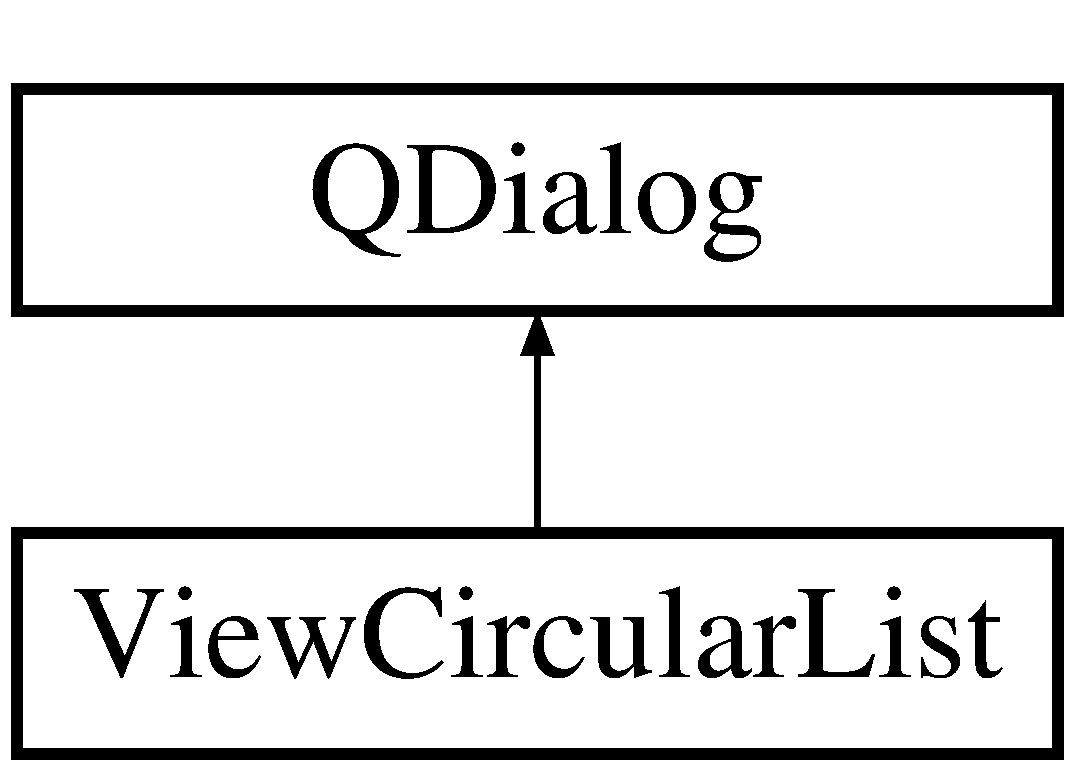
\includegraphics[height=2.000000cm]{class_view_circular_list}
\end{center}
\end{figure}
\subsection*{Métodos públicos}
\begin{DoxyCompactItemize}
\item 
\mbox{\hyperlink{class_view_circular_list_a5c2f50cf83d080aef15678bcf9b51ee1}{View\+Circular\+List}} (Q\+Widget $\ast$parent=0)
\item 
\mbox{\hyperlink{class_view_circular_list_a3daf1e98019445c90f6b12d5e0083092}{$\sim$\+View\+Circular\+List}} ()
\end{DoxyCompactItemize}
\subsection*{Atributos públicos}
\begin{DoxyCompactItemize}
\item 
\mbox{\hyperlink{class_circular_list}{Circular\+List}} $\ast$ \mbox{\hyperlink{class_view_circular_list_a10f35f007af0844f3966340a74542d3f}{lista}}
\item 
int \mbox{\hyperlink{class_view_circular_list_a9dca774f51b7b6bab8515b862774315f}{posx}}
\end{DoxyCompactItemize}


\subsection{Descripción detallada}
The \mbox{\hyperlink{class_view_circular_list}{View\+Circular\+List}} class Ventana De la Lista Circular. 

\subsection{Documentación del constructor y destructor}
\mbox{\Hypertarget{class_view_circular_list_a5c2f50cf83d080aef15678bcf9b51ee1}\label{class_view_circular_list_a5c2f50cf83d080aef15678bcf9b51ee1}} 
\index{View\+Circular\+List@{View\+Circular\+List}!View\+Circular\+List@{View\+Circular\+List}}
\index{View\+Circular\+List@{View\+Circular\+List}!View\+Circular\+List@{View\+Circular\+List}}
\subsubsection{\texorpdfstring{View\+Circular\+List()}{ViewCircularList()}}
{\footnotesize\ttfamily View\+Circular\+List\+::\+View\+Circular\+List (\begin{DoxyParamCaption}\item[{Q\+Widget $\ast$}]{parent = {\ttfamily 0} }\end{DoxyParamCaption})\hspace{0.3cm}{\ttfamily [explicit]}}

\mbox{\Hypertarget{class_view_circular_list_a3daf1e98019445c90f6b12d5e0083092}\label{class_view_circular_list_a3daf1e98019445c90f6b12d5e0083092}} 
\index{View\+Circular\+List@{View\+Circular\+List}!````~View\+Circular\+List@{$\sim$\+View\+Circular\+List}}
\index{````~View\+Circular\+List@{$\sim$\+View\+Circular\+List}!View\+Circular\+List@{View\+Circular\+List}}
\subsubsection{\texorpdfstring{$\sim$\+View\+Circular\+List()}{~ViewCircularList()}}
{\footnotesize\ttfamily View\+Circular\+List\+::$\sim$\+View\+Circular\+List (\begin{DoxyParamCaption}{ }\end{DoxyParamCaption})}



\subsection{Documentación de los datos miembro}
\mbox{\Hypertarget{class_view_circular_list_a10f35f007af0844f3966340a74542d3f}\label{class_view_circular_list_a10f35f007af0844f3966340a74542d3f}} 
\index{View\+Circular\+List@{View\+Circular\+List}!lista@{lista}}
\index{lista@{lista}!View\+Circular\+List@{View\+Circular\+List}}
\subsubsection{\texorpdfstring{lista}{lista}}
{\footnotesize\ttfamily \mbox{\hyperlink{class_circular_list}{Circular\+List}}$\ast$ View\+Circular\+List\+::lista}

\mbox{\Hypertarget{class_view_circular_list_a9dca774f51b7b6bab8515b862774315f}\label{class_view_circular_list_a9dca774f51b7b6bab8515b862774315f}} 
\index{View\+Circular\+List@{View\+Circular\+List}!posx@{posx}}
\index{posx@{posx}!View\+Circular\+List@{View\+Circular\+List}}
\subsubsection{\texorpdfstring{posx}{posx}}
{\footnotesize\ttfamily int View\+Circular\+List\+::posx}



La documentación para esta clase fue generada a partir de los siguientes ficheros\+:\begin{DoxyCompactItemize}
\item 
\mbox{\hyperlink{viewcircularlist_8h}{viewcircularlist.\+h}}\item 
\mbox{\hyperlink{viewcircularlist_8cpp}{viewcircularlist.\+cpp}}\end{DoxyCompactItemize}

\hypertarget{class_view_tree}{}\section{Referencia de la Clase View\+Tree}
\label{class_view_tree}\index{View\+Tree@{View\+Tree}}


The \mbox{\hyperlink{class_view_tree}{View\+Tree}} class clase que se encarga de la ventana del Arbol binario.  




{\ttfamily \#include $<$viewtree.\+h$>$}

Diagrama de herencias de View\+Tree\begin{figure}[H]
\begin{center}
\leavevmode
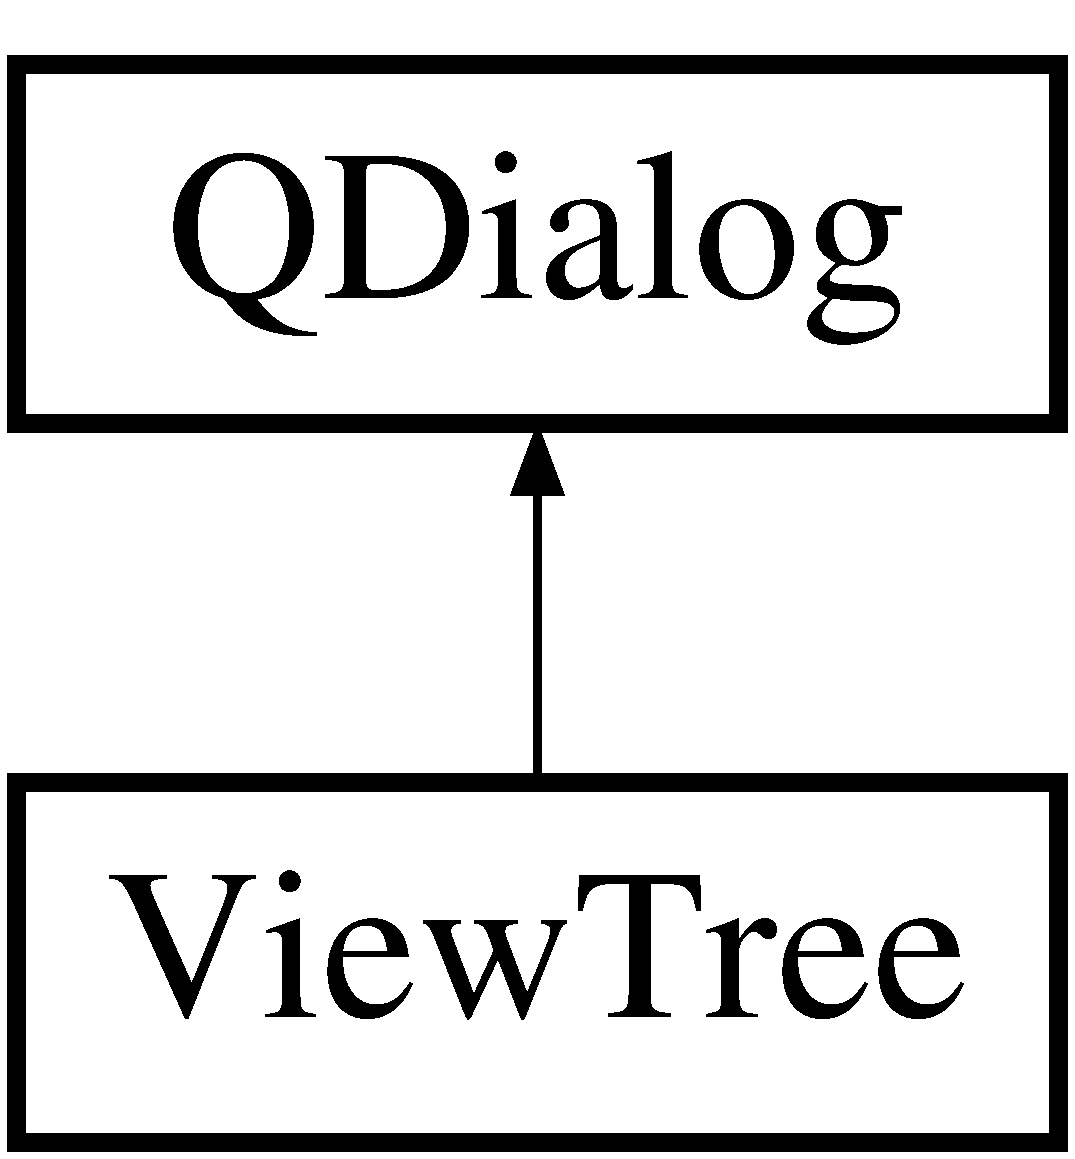
\includegraphics[height=2.000000cm]{class_view_tree}
\end{center}
\end{figure}
\subsection*{Métodos públicos}
\begin{DoxyCompactItemize}
\item 
\mbox{\hyperlink{class_view_tree_ab2903b9d0a3b1b9a147a5b1e2206ac0e}{View\+Tree}} (Q\+Widget $\ast$parent=0)
\item 
\mbox{\hyperlink{class_view_tree_a0ad5e737640d9b992b39088dbfe9f291}{$\sim$\+View\+Tree}} ()
\end{DoxyCompactItemize}


\subsection{Descripción detallada}
The \mbox{\hyperlink{class_view_tree}{View\+Tree}} class clase que se encarga de la ventana del Arbol binario. 

\subsection{Documentación del constructor y destructor}
\mbox{\Hypertarget{class_view_tree_ab2903b9d0a3b1b9a147a5b1e2206ac0e}\label{class_view_tree_ab2903b9d0a3b1b9a147a5b1e2206ac0e}} 
\index{View\+Tree@{View\+Tree}!View\+Tree@{View\+Tree}}
\index{View\+Tree@{View\+Tree}!View\+Tree@{View\+Tree}}
\subsubsection{\texorpdfstring{View\+Tree()}{ViewTree()}}
{\footnotesize\ttfamily View\+Tree\+::\+View\+Tree (\begin{DoxyParamCaption}\item[{Q\+Widget $\ast$}]{parent = {\ttfamily 0} }\end{DoxyParamCaption})\hspace{0.3cm}{\ttfamily [explicit]}}

\mbox{\Hypertarget{class_view_tree_a0ad5e737640d9b992b39088dbfe9f291}\label{class_view_tree_a0ad5e737640d9b992b39088dbfe9f291}} 
\index{View\+Tree@{View\+Tree}!````~View\+Tree@{$\sim$\+View\+Tree}}
\index{````~View\+Tree@{$\sim$\+View\+Tree}!View\+Tree@{View\+Tree}}
\subsubsection{\texorpdfstring{$\sim$\+View\+Tree()}{~ViewTree()}}
{\footnotesize\ttfamily View\+Tree\+::$\sim$\+View\+Tree (\begin{DoxyParamCaption}{ }\end{DoxyParamCaption})}



La documentación para esta clase fue generada a partir de los siguientes ficheros\+:\begin{DoxyCompactItemize}
\item 
\mbox{\hyperlink{viewtree_8h}{viewtree.\+h}}\item 
\mbox{\hyperlink{viewtree_8cpp}{viewtree.\+cpp}}\end{DoxyCompactItemize}

\chapter{Documentación de archivos}
\hypertarget{binarytree_8h}{}\section{Referencia del Archivo binarytree.\+h}
\label{binarytree_8h}\index{binarytree.\+h@{binarytree.\+h}}


Archivo que tiene lo referente al arbol binario.  


{\ttfamily \#include $<$iostream$>$}\newline
{\ttfamily \#include $<$string$>$}\newline
{\ttfamily \#include \char`\"{}treenode.\+h\char`\"{}}\newline
\subsection*{Clases}
\begin{DoxyCompactItemize}
\item 
class \mbox{\hyperlink{class_binary_tree}{Binary\+Tree}}
\begin{DoxyCompactList}\small\item\em The \mbox{\hyperlink{class_binary_tree}{Binary\+Tree}} class clase que maneja la estructura del arbol binario. \end{DoxyCompactList}\end{DoxyCompactItemize}


\subsection{Descripción detallada}
Archivo que tiene lo referente al arbol binario. 

\begin{DoxyVersion}{Versión}
1.\+0 
\end{DoxyVersion}
\begin{DoxyDate}{Fecha}
5/3/18 
\end{DoxyDate}
\begin{DoxyAuthor}{Autor}
Oscar Isaac Porras Perez  Binary Tree 
\end{DoxyAuthor}

\hypertarget{circularlist_8h}{}\section{Referencia del Archivo circularlist.\+h}
\label{circularlist_8h}\index{circularlist.\+h@{circularlist.\+h}}


Estructura de datos lista circular.  


{\ttfamily \#include \char`\"{}Nodo\+Lista\+Circular.\+h\char`\"{}}\newline
{\ttfamily \#include \char`\"{}Q\+String\char`\"{}}\newline
{\ttfamily \#include $<$iostream$>$}\newline
{\ttfamily \#include $<$string$>$}\newline
{\ttfamily \#include $<$stdio.\+h$>$}\newline
\subsection*{Clases}
\begin{DoxyCompactItemize}
\item 
class \mbox{\hyperlink{class_circular_list}{Circular\+List}}
\begin{DoxyCompactList}\small\item\em The \mbox{\hyperlink{class_circular_list}{Circular\+List}} class clase que contiene la estructura de datos de la lista circular. \end{DoxyCompactList}\end{DoxyCompactItemize}


\subsection{Descripción detallada}
Estructura de datos lista circular. 

\begin{DoxyVersion}{Versión}
1.\+0 
\end{DoxyVersion}
\begin{DoxyDate}{Fecha}
5/3/18 
\end{DoxyDate}
\begin{DoxyAuthor}{Autor}
Oscar Isaac Porras Perez  \mbox{\hyperlink{class_circular_list}{Circular\+List}} 
\end{DoxyAuthor}

\hypertarget{doblelinkedlist_8h}{}\section{Referencia del Archivo doblelinkedlist.\+h}
\label{doblelinkedlist_8h}\index{doblelinkedlist.\+h@{doblelinkedlist.\+h}}


Estructura de datos lista doblemente enlanzada.  


{\ttfamily \#include \char`\"{}nododobleenlazado.\+h\char`\"{}}\newline
{\ttfamily \#include \char`\"{}Q\+String\char`\"{}}\newline
{\ttfamily \#include $<$iostream$>$}\newline
{\ttfamily \#include $<$string$>$}\newline
\subsection*{Clases}
\begin{DoxyCompactItemize}
\item 
class \mbox{\hyperlink{class_doble_linked_list}{Doble\+Linked\+List}}
\begin{DoxyCompactList}\small\item\em The \mbox{\hyperlink{class_doble_linked_list}{Doble\+Linked\+List}} class clase que contiene la estructura de las listas doblemente enlazadas. \end{DoxyCompactList}\end{DoxyCompactItemize}


\subsection{Descripción detallada}
Estructura de datos lista doblemente enlanzada. 

\begin{DoxyVersion}{Versión}
1.\+0 
\end{DoxyVersion}
\begin{DoxyDate}{Fecha}
5/3/18 
\end{DoxyDate}
\begin{DoxyAuthor}{Autor}
Oscar Isaac Porras Perez  \mbox{\hyperlink{class_doble_linked_list}{Doble\+Linked\+List}} 
\end{DoxyAuthor}

\hypertarget{enlazadadoble_8cpp}{}\section{Referencia del Archivo enlazadadoble.\+cpp}
\label{enlazadadoble_8cpp}\index{enlazadadoble.\+cpp@{enlazadadoble.\+cpp}}
{\ttfamily \#include \char`\"{}enlazadadoble.\+h\char`\"{}}\newline
{\ttfamily \#include \char`\"{}ui\+\_\+enlazadadoble.\+h\char`\"{}}\newline
{\ttfamily \#include \char`\"{}Q\+Paint\+Event\char`\"{}}\newline
{\ttfamily \#include \char`\"{}Q\+Painter\char`\"{}}\newline
{\ttfamily \#include \char`\"{}Q\+Dialog\char`\"{}}\newline
{\ttfamily \#include \char`\"{}Qt\+Gui\char`\"{}}\newline
{\ttfamily \#include \char`\"{}Qt\+Core\char`\"{}}\newline
{\ttfamily \#include \char`\"{}Q\+Graphics\+Scene\char`\"{}}\newline
{\ttfamily \#include $<$Q\+Text\+Edit$>$}\newline

\hypertarget{enlazadadoble_8h}{}\section{Referencia del Archivo enlazadadoble.\+h}
\label{enlazadadoble_8h}\index{enlazadadoble.\+h@{enlazadadoble.\+h}}


contiene lo referente a la ventana de la lista doblemente enlazada  


{\ttfamily \#include $<$iostream$>$}\newline
{\ttfamily \#include \char`\"{}Q\+Paint\+Event\char`\"{}}\newline
{\ttfamily \#include \char`\"{}Q\+Painter\char`\"{}}\newline
{\ttfamily \#include \char`\"{}Q\+Dialog\char`\"{}}\newline
{\ttfamily \#include \char`\"{}Qt\+Gui\char`\"{}}\newline
{\ttfamily \#include \char`\"{}Qt\+Core\char`\"{}}\newline
{\ttfamily \#include \char`\"{}Q\+Graphics\+Scene\char`\"{}}\newline
{\ttfamily \#include $<$Q\+Text\+Edit$>$}\newline
{\ttfamily \#include \char`\"{}doblelinkedlist.\+h\char`\"{}}\newline
\subsection*{Clases}
\begin{DoxyCompactItemize}
\item 
class \mbox{\hyperlink{class_enlazada_doble}{Enlazada\+Doble}}
\begin{DoxyCompactList}\small\item\em The \mbox{\hyperlink{class_enlazada_doble}{Enlazada\+Doble}} class clase que contiene lo referente a la ventana de la lista doblemente enlazada. \end{DoxyCompactList}\end{DoxyCompactItemize}
\subsection*{Namespaces}
\begin{DoxyCompactItemize}
\item 
 \mbox{\hyperlink{namespace_ui}{Ui}}
\end{DoxyCompactItemize}


\subsection{Descripción detallada}
contiene lo referente a la ventana de la lista doblemente enlazada 

\begin{DoxyVersion}{Versión}
1.\+0 
\end{DoxyVersion}
\begin{DoxyDate}{Fecha}
5/3/18 
\end{DoxyDate}
\begin{DoxyAuthor}{Autor}
Oscar Isaac Porras Perez  Enlazada Doble 
\end{DoxyAuthor}

\hypertarget{listasimple_8cpp}{}\section{Referencia del Archivo listasimple.\+cpp}
\label{listasimple_8cpp}\index{listasimple.\+cpp@{listasimple.\+cpp}}
{\ttfamily \#include \char`\"{}listasimple.\+h\char`\"{}}\newline
{\ttfamily \#include \char`\"{}ui\+\_\+listasimple.\+h\char`\"{}}\newline
{\ttfamily \#include \char`\"{}Q\+Paint\+Event\char`\"{}}\newline
{\ttfamily \#include \char`\"{}Q\+Painter\char`\"{}}\newline
{\ttfamily \#include \char`\"{}Q\+Dialog\char`\"{}}\newline
{\ttfamily \#include \char`\"{}Qt\+Gui\char`\"{}}\newline
{\ttfamily \#include \char`\"{}Qt\+Core\char`\"{}}\newline
{\ttfamily \#include \char`\"{}Q\+Graphics\+Scene\char`\"{}}\newline
{\ttfamily \#include $<$Q\+Text\+Edit$>$}\newline
{\ttfamily \#include \char`\"{}simplelinkedlist.\+h\char`\"{}}\newline

\hypertarget{listasimple_8h}{}\section{Referencia del Archivo listasimple.\+h}
\label{listasimple_8h}\index{listasimple.\+h@{listasimple.\+h}}


contiene lo referente a la ventana de la lista simple  


{\ttfamily \#include $<$Q\+Dialog$>$}\newline
{\ttfamily \#include \char`\"{}Q\+Graphics\+Scene\char`\"{}}\newline
{\ttfamily \#include \char`\"{}simplelinkedlist.\+h\char`\"{}}\newline
\subsection*{Clases}
\begin{DoxyCompactItemize}
\item 
class \mbox{\hyperlink{class_lista_simple}{Lista\+Simple}}
\begin{DoxyCompactList}\small\item\em The \mbox{\hyperlink{class_lista_simple}{Lista\+Simple}} class clase que contiene lo referente a la ventana de la lista simple. \end{DoxyCompactList}\end{DoxyCompactItemize}
\subsection*{Namespaces}
\begin{DoxyCompactItemize}
\item 
 \mbox{\hyperlink{namespace_ui}{Ui}}
\end{DoxyCompactItemize}


\subsection{Descripción detallada}
contiene lo referente a la ventana de la lista simple 

\begin{DoxyVersion}{Versión}
1.\+0 
\end{DoxyVersion}
\begin{DoxyDate}{Fecha}
5/3/18 
\end{DoxyDate}
\begin{DoxyAuthor}{Autor}
Oscar Isaac Porras Perez  \mbox{\hyperlink{class_lista_simple}{Lista\+Simple}} 
\end{DoxyAuthor}

\hypertarget{main_8cpp}{}\section{Referencia del Archivo main.\+cpp}
\label{main_8cpp}\index{main.\+cpp@{main.\+cpp}}
{\ttfamily \#include \char`\"{}mainwindow.\+h\char`\"{}}\newline
{\ttfamily \#include $<$Q\+Application$>$}\newline
\subsection*{Funciones}
\begin{DoxyCompactItemize}
\item 
int \mbox{\hyperlink{main_8cpp_a0ddf1224851353fc92bfbff6f499fa97}{main}} (int argc, char $\ast$argv\mbox{[}$\,$\mbox{]})
\end{DoxyCompactItemize}


\subsection{Documentación de las funciones}
\mbox{\Hypertarget{main_8cpp_a0ddf1224851353fc92bfbff6f499fa97}\label{main_8cpp_a0ddf1224851353fc92bfbff6f499fa97}} 
\index{main.\+cpp@{main.\+cpp}!main@{main}}
\index{main@{main}!main.\+cpp@{main.\+cpp}}
\subsubsection{\texorpdfstring{main()}{main()}}
{\footnotesize\ttfamily int main (\begin{DoxyParamCaption}\item[{int}]{argc,  }\item[{char $\ast$}]{argv\mbox{[}$\,$\mbox{]} }\end{DoxyParamCaption})}


\hypertarget{mainwindow_8cpp}{}\section{Referencia del Archivo mainwindow.\+cpp}
\label{mainwindow_8cpp}\index{mainwindow.\+cpp@{mainwindow.\+cpp}}
{\ttfamily \#include \char`\"{}mainwindow.\+h\char`\"{}}\newline
{\ttfamily \#include \char`\"{}ui\+\_\+mainwindow.\+h\char`\"{}}\newline
{\ttfamily \#include \char`\"{}listasimple.\+h\char`\"{}}\newline
{\ttfamily \#include \char`\"{}enlazadadoble.\+h\char`\"{}}\newline
{\ttfamily \#include \char`\"{}viewcircularlist.\+h\char`\"{}}\newline
{\ttfamily \#include \char`\"{}viewtree.\+h\char`\"{}}\newline

\hypertarget{mainwindow_8h}{}\section{Referencia del Archivo mainwindow.\+h}
\label{mainwindow_8h}\index{mainwindow.\+h@{mainwindow.\+h}}


controla todo lo referente a lo que se encuentra en la ventana principal  


{\ttfamily \#include $<$Q\+Main\+Window$>$}\newline
\subsection*{Clases}
\begin{DoxyCompactItemize}
\item 
class \mbox{\hyperlink{class_main_window}{Main\+Window}}
\begin{DoxyCompactList}\small\item\em The \mbox{\hyperlink{class_main_window}{Main\+Window}} class Esta clase controla todo lo referente a lo que se encuentra en la ventana inicial. \end{DoxyCompactList}\end{DoxyCompactItemize}
\subsection*{Namespaces}
\begin{DoxyCompactItemize}
\item 
 \mbox{\hyperlink{namespace_ui}{Ui}}
\end{DoxyCompactItemize}


\subsection{Descripción detallada}
controla todo lo referente a lo que se encuentra en la ventana principal 

\begin{DoxyVersion}{Versión}
1.\+0 
\end{DoxyVersion}
\begin{DoxyDate}{Fecha}
5/3/18 
\end{DoxyDate}
\begin{DoxyAuthor}{Autor}
Oscar Isaac Porras Perez  Binary Tree 
\end{DoxyAuthor}

\hypertarget{nododobleenlazado_8h}{}\section{Referencia del Archivo nododobleenlazado.\+h}
\label{nododobleenlazado_8h}\index{nododobleenlazado.\+h@{nododobleenlazado.\+h}}


Estructura de datos nodo para lista doble enlazada.  


{\ttfamily \#include \char`\"{}Q\+String\char`\"{}}\newline
{\ttfamily \#include $<$iostream$>$}\newline
{\ttfamily \#include $<$string$>$}\newline
\subsection*{Clases}
\begin{DoxyCompactItemize}
\item 
class \mbox{\hyperlink{class_nodo_doble_enlazado}{Nodo\+Doble\+Enlazado}}
\begin{DoxyCompactList}\small\item\em The \mbox{\hyperlink{class_nodo_doble_enlazado}{Nodo\+Doble\+Enlazado}} class Estructura de datos nodo para lista doble enlazada. \end{DoxyCompactList}\end{DoxyCompactItemize}
\subsection*{defines}
\begin{DoxyCompactItemize}
\item 
\#define \mbox{\hyperlink{nododobleenlazado_8h_ac97b8ee753e4405397a42ad5799b0f9e}{null}}~0;
\end{DoxyCompactItemize}


\subsection{Descripción detallada}
Estructura de datos nodo para lista doble enlazada. 

\begin{DoxyVersion}{Versión}
1.\+0 
\end{DoxyVersion}
\begin{DoxyDate}{Fecha}
5/3/18 
\end{DoxyDate}
\begin{DoxyAuthor}{Autor}
Oscar Isaac Porras Perez  Nodo para la lista doble enlazada 
\end{DoxyAuthor}


\subsection{Documentación de los \textquotesingle{}defines\textquotesingle{}}
\mbox{\Hypertarget{nododobleenlazado_8h_ac97b8ee753e4405397a42ad5799b0f9e}\label{nododobleenlazado_8h_ac97b8ee753e4405397a42ad5799b0f9e}} 
\index{nododobleenlazado.\+h@{nododobleenlazado.\+h}!null@{null}}
\index{null@{null}!nododobleenlazado.\+h@{nododobleenlazado.\+h}}
\subsubsection{\texorpdfstring{null}{null}}
{\footnotesize\ttfamily \#define null~0;}


\hypertarget{nodolistacircular_8h}{}\section{Referencia del Archivo nodolistacircular.\+h}
\label{nodolistacircular_8h}\index{nodolistacircular.\+h@{nodolistacircular.\+h}}


Estructura del nodo de la lista circular.  


{\ttfamily \#include \char`\"{}Q\+String\char`\"{}}\newline
{\ttfamily \#include $<$iostream$>$}\newline
{\ttfamily \#include $<$string$>$}\newline
\subsection*{Clases}
\begin{DoxyCompactItemize}
\item 
class \mbox{\hyperlink{class_nodo_lista_circular}{Nodo\+Lista\+Circular}}
\begin{DoxyCompactList}\small\item\em The \mbox{\hyperlink{class_nodo_lista_circular}{Nodo\+Lista\+Circular}} class Estructura del nodo de la lista circular. \end{DoxyCompactList}\end{DoxyCompactItemize}
\subsection*{defines}
\begin{DoxyCompactItemize}
\item 
\#define \mbox{\hyperlink{nodolistacircular_8h_ac97b8ee753e4405397a42ad5799b0f9e}{null}}~0;
\end{DoxyCompactItemize}


\subsection{Descripción detallada}
Estructura del nodo de la lista circular. 

\begin{DoxyVersion}{Versión}
1.\+0 
\end{DoxyVersion}
\begin{DoxyDate}{Fecha}
5/3/18 
\end{DoxyDate}
\begin{DoxyAuthor}{Autor}
Oscar Isaac Porras Perez  Nodo Lista Circular 
\end{DoxyAuthor}


\subsection{Documentación de los \textquotesingle{}defines\textquotesingle{}}
\mbox{\Hypertarget{nodolistacircular_8h_ac97b8ee753e4405397a42ad5799b0f9e}\label{nodolistacircular_8h_ac97b8ee753e4405397a42ad5799b0f9e}} 
\index{nodolistacircular.\+h@{nodolistacircular.\+h}!null@{null}}
\index{null@{null}!nodolistacircular.\+h@{nodolistacircular.\+h}}
\subsubsection{\texorpdfstring{null}{null}}
{\footnotesize\ttfamily \#define null~0;}


\hypertarget{nodosimple_8h}{}\section{Referencia del Archivo nodosimple.\+h}
\label{nodosimple_8h}\index{nodosimple.\+h@{nodosimple.\+h}}


Estructura del nodo de la lista simple.  


{\ttfamily \#include \char`\"{}Q\+String\char`\"{}}\newline
{\ttfamily \#include $<$iostream$>$}\newline
{\ttfamily \#include $<$string$>$}\newline
\subsection*{Clases}
\begin{DoxyCompactItemize}
\item 
class \mbox{\hyperlink{class_nodo_simple}{Nodo\+Simple}}
\begin{DoxyCompactList}\small\item\em The \mbox{\hyperlink{class_nodo_simple}{Nodo\+Simple}} class Estructura del nodo de la lista simple. \end{DoxyCompactList}\end{DoxyCompactItemize}
\subsection*{defines}
\begin{DoxyCompactItemize}
\item 
\#define \mbox{\hyperlink{nodosimple_8h_ac97b8ee753e4405397a42ad5799b0f9e}{null}}~0;
\end{DoxyCompactItemize}


\subsection{Descripción detallada}
Estructura del nodo de la lista simple. 

\begin{DoxyVersion}{Versión}
1.\+0 
\end{DoxyVersion}
\begin{DoxyDate}{Fecha}
5/3/18 
\end{DoxyDate}
\begin{DoxyAuthor}{Autor}
Oscar Isaac Porras Perez  Nodo Simple 
\end{DoxyAuthor}


\subsection{Documentación de los \textquotesingle{}defines\textquotesingle{}}
\mbox{\Hypertarget{nodosimple_8h_ac97b8ee753e4405397a42ad5799b0f9e}\label{nodosimple_8h_ac97b8ee753e4405397a42ad5799b0f9e}} 
\index{nodosimple.\+h@{nodosimple.\+h}!null@{null}}
\index{null@{null}!nodosimple.\+h@{nodosimple.\+h}}
\subsubsection{\texorpdfstring{null}{null}}
{\footnotesize\ttfamily \#define null~0;}


\hypertarget{simplelinkedlist_8h}{}\section{Referencia del Archivo simplelinkedlist.\+h}
\label{simplelinkedlist_8h}\index{simplelinkedlist.\+h@{simplelinkedlist.\+h}}


Estructura de la lista simple.  


{\ttfamily \#include \char`\"{}Q\+String\char`\"{}}\newline
{\ttfamily \#include \char`\"{}nodosimple.\+h\char`\"{}}\newline
\subsection*{Clases}
\begin{DoxyCompactItemize}
\item 
class \mbox{\hyperlink{class_simple_linked_list}{Simple\+Linked\+List}}
\begin{DoxyCompactList}\small\item\em The \mbox{\hyperlink{class_simple_linked_list}{Simple\+Linked\+List}} class Estructura de la lista simple. \end{DoxyCompactList}\end{DoxyCompactItemize}
\subsection*{defines}
\begin{DoxyCompactItemize}
\item 
\#define \mbox{\hyperlink{simplelinkedlist_8h_ac97b8ee753e4405397a42ad5799b0f9e}{null}}~0;
\end{DoxyCompactItemize}


\subsection{Descripción detallada}
Estructura de la lista simple. 

\begin{DoxyVersion}{Versión}
1.\+0 
\end{DoxyVersion}
\begin{DoxyDate}{Fecha}
5/3/18 
\end{DoxyDate}
\begin{DoxyAuthor}{Autor}
Oscar Isaac Porras Perez  Simple Linked List 
\end{DoxyAuthor}


\subsection{Documentación de los \textquotesingle{}defines\textquotesingle{}}
\mbox{\Hypertarget{simplelinkedlist_8h_ac97b8ee753e4405397a42ad5799b0f9e}\label{simplelinkedlist_8h_ac97b8ee753e4405397a42ad5799b0f9e}} 
\index{simplelinkedlist.\+h@{simplelinkedlist.\+h}!null@{null}}
\index{null@{null}!simplelinkedlist.\+h@{simplelinkedlist.\+h}}
\subsubsection{\texorpdfstring{null}{null}}
{\footnotesize\ttfamily \#define null~0;}


\hypertarget{treenode_8h}{}\section{Referencia del Archivo treenode.\+h}
\label{treenode_8h}\index{treenode.\+h@{treenode.\+h}}


Estructura del nodo para el arbol.  


{\ttfamily \#include $<$iostream$>$}\newline
{\ttfamily \#include $<$string$>$}\newline
\subsection*{Clases}
\begin{DoxyCompactItemize}
\item 
class \mbox{\hyperlink{class_tree_node}{Tree\+Node}}
\begin{DoxyCompactList}\small\item\em The \mbox{\hyperlink{class_tree_node}{Tree\+Node}} class Estructura del nodo para el arbol. \end{DoxyCompactList}\end{DoxyCompactItemize}


\subsection{Descripción detallada}
Estructura del nodo para el arbol. 

\begin{DoxyVersion}{Versión}
1.\+0 
\end{DoxyVersion}
\begin{DoxyDate}{Fecha}
5/3/18 
\end{DoxyDate}
\begin{DoxyAuthor}{Autor}
Oscar Isaac Porras Perez  Tree Node 
\end{DoxyAuthor}

\hypertarget{viewcircularlist_8cpp}{}\section{Referencia del Archivo viewcircularlist.\+cpp}
\label{viewcircularlist_8cpp}\index{viewcircularlist.\+cpp@{viewcircularlist.\+cpp}}
{\ttfamily \#include \char`\"{}viewcircularlist.\+h\char`\"{}}\newline
{\ttfamily \#include \char`\"{}ui\+\_\+viewcircularlist.\+h\char`\"{}}\newline
{\ttfamily \#include \char`\"{}Q\+Paint\+Event\char`\"{}}\newline
{\ttfamily \#include \char`\"{}Q\+Painter\char`\"{}}\newline
{\ttfamily \#include \char`\"{}Q\+Dialog\char`\"{}}\newline
{\ttfamily \#include \char`\"{}Qt\+Gui\char`\"{}}\newline
{\ttfamily \#include \char`\"{}Qt\+Core\char`\"{}}\newline
{\ttfamily \#include \char`\"{}Q\+Graphics\+Scene\char`\"{}}\newline
{\ttfamily \#include $<$Q\+Text\+Edit$>$}\newline
{\ttfamily \#include \char`\"{}circularlist.\+h\char`\"{}}\newline

\hypertarget{viewcircularlist_8h}{}\section{Referencia del Archivo viewcircularlist.\+h}
\label{viewcircularlist_8h}\index{viewcircularlist.\+h@{viewcircularlist.\+h}}


controla todo lo referente a la ventana De la Lista Circular  


{\ttfamily \#include $<$Q\+Dialog$>$}\newline
{\ttfamily \#include \char`\"{}Q\+Graphics\+Scene\char`\"{}}\newline
{\ttfamily \#include \char`\"{}circularlist.\+h\char`\"{}}\newline
\subsection*{Clases}
\begin{DoxyCompactItemize}
\item 
class \mbox{\hyperlink{class_view_circular_list}{View\+Circular\+List}}
\begin{DoxyCompactList}\small\item\em The \mbox{\hyperlink{class_view_circular_list}{View\+Circular\+List}} class Ventana De la Lista Circular. \end{DoxyCompactList}\end{DoxyCompactItemize}
\subsection*{Namespaces}
\begin{DoxyCompactItemize}
\item 
 \mbox{\hyperlink{namespace_ui}{Ui}}
\end{DoxyCompactItemize}


\subsection{Descripción detallada}
controla todo lo referente a la ventana De la Lista Circular 

\begin{DoxyVersion}{Versión}
1.\+0 
\end{DoxyVersion}
\begin{DoxyDate}{Fecha}
5/3/18 
\end{DoxyDate}
\begin{DoxyAuthor}{Autor}
Oscar Isaac Porras Perez  Ventana De la Lista Circular 
\end{DoxyAuthor}

\hypertarget{viewtree_8cpp}{}\section{Referencia del Archivo viewtree.\+cpp}
\label{viewtree_8cpp}\index{viewtree.\+cpp@{viewtree.\+cpp}}
{\ttfamily \#include \char`\"{}viewtree.\+h\char`\"{}}\newline
{\ttfamily \#include \char`\"{}ui\+\_\+viewtree.\+h\char`\"{}}\newline
{\ttfamily \#include \char`\"{}binarytree.\+h\char`\"{}}\newline

\hypertarget{viewtree_8h}{}\section{Referencia del Archivo viewtree.\+h}
\label{viewtree_8h}\index{viewtree.\+h@{viewtree.\+h}}


contiene todo lo referente a la ventana del arbol binario  


{\ttfamily \#include \char`\"{}binarytree.\+h\char`\"{}}\newline
{\ttfamily \#include \char`\"{}Q\+Graphics\+Scene\char`\"{}}\newline
{\ttfamily \#include \char`\"{}treenode.\+h\char`\"{}}\newline
{\ttfamily \#include $<$Q\+Dialog$>$}\newline
\subsection*{Clases}
\begin{DoxyCompactItemize}
\item 
class \mbox{\hyperlink{class_view_tree}{View\+Tree}}
\begin{DoxyCompactList}\small\item\em The \mbox{\hyperlink{class_view_tree}{View\+Tree}} class clase que se encarga de la ventana del Arbol binario. \end{DoxyCompactList}\end{DoxyCompactItemize}
\subsection*{Namespaces}
\begin{DoxyCompactItemize}
\item 
 \mbox{\hyperlink{namespace_ui}{Ui}}
\end{DoxyCompactItemize}


\subsection{Descripción detallada}
contiene todo lo referente a la ventana del arbol binario 

\begin{DoxyVersion}{Versión}
1.\+0 
\end{DoxyVersion}
\begin{DoxyDate}{Fecha}
5/3/18 
\end{DoxyDate}
\begin{DoxyAuthor}{Autor}
Oscar Isaac Porras Perez  \mbox{\hyperlink{class_view_tree}{View\+Tree}} 
\end{DoxyAuthor}

%--- End generated contents ---

% Index
\backmatter
\newpage
\phantomsection
\clearemptydoublepage
\addcontentsline{toc}{chapter}{Índice}
\printindex

\end{document}
